\nonstopmode
\documentclass[10pt, a4paper]{article}
\parindent=20pt
\parskip=8pt
\usepackage[width=15.5cm, left=3cm, top=2.5cm, height= 24.5cm]{geometry}
\usepackage[spanish]{babel}
\usepackage[utf8]{inputenc}
\usepackage{fancyhdr}
\usepackage{multirow}
\usepackage{rotating}
\usepackage{indentfirst}
\usepackage{latexsym}
\usepackage{caratula}
\usepackage{gnuplottex}
\usepackage{epsfig}
\usepackage{lastpage}
\usepackage{amsfonts}
\usepackage{listings}
\lstset{language=C}
\usepackage[export]{adjustbox}
\usepackage{pdfpages}
\usepackage{amsmath}
\usepackage{verbatim}
\usepackage[ruled,vlined,linesnumbered]{algorithm2e}
\usepackage{graphicx}
\usepackage{float}
\usepackage{color}

\graphicspath{{imgs/}}

% Acomodo fancyhdr.
\pagestyle{fancy}
\thispagestyle{fancy}
\addtolength{\headheight}{1pt}
\lhead{Organización del Computador II}
\rhead{TP Final}
\cfoot{\thepage /\pageref{LastPage}}
\renewcommand{\footrulewidth}{0.4pt}
\renewcommand{\thesubsubsection}{\thesubsection.\alph{subsubsection}}


\author{Organización del Computador II, DC, UBA.}
\date{}
\title{}

\begin{document}
	
\thispagestyle{empty}
\materia{Organización del Computador 2}
\submateria{Trabajo Pr\'actico Final}
\titulo{Reconocimiento Óptico de Caracteres.}
\integrante{Izcovich, Sabrina}{550/11}{sizcovich@gmail.com}
\integrante{Vita, Sebastián}{149/11}{sebastian\_vita@yahoo.com.ar}

\maketitle

\tableofcontents
\newpage

\section{Introducci\'on}
El reconocimiento óptico de caracteres (OCR, por sus siglas en inglés) es el proceso por el cual se traducen o convierten imágenes de dígitos o caracteres (sean éstos manuscritos o de alguna tipografía especial) a un formato representable por nuestra computadora (por ejemplo, ASCII). Esta tarea puede ser más sencilla (por ejemplo, cuando tratamos de determinar el texto escrito en una versión escaneada a buena resolución de un libro) o tornarse casi imposible (por ejemplo, cuando intentamos leer la receta de un médico).\newline
\newline
Este trabajo consiste en una implementación de un método de reconocimiento de dígitos manuscritos en $C$ y $Assembler$. Dichas implementaciones consisten en un programa encargado de leer imágenes que, a partir de la descomposición en valores singulares, logra determinar de qué dígito se trata. Para que las pruebas fueran posibles, utilizamos la base de datos MNIST que nos proporcionó una gran cantidad de imágenes de cada dígito que luego serían comparadas con el dígito a definir. Para alcanzar nuestro objetivo debimos hallar los autovalores y autovectores de la matriz de covarianza de la base de datos. Para ello, utilizamos el Método de Factorización QR.

Por otro lado, debimos analizar la performance de un procesador al hacer uso de las operaciones SIMD. Para ello, realizamos comparaciones de velocidad entre los dos tipos de implementaciones realizados utilizando la herramienta Time Stamp Counter (TSC) del procesador y sacamos conclusiones al respecto.

\section{Introducci\'on te\'orica}
Para la realización del estudio de señales, utilizamos los siguientes conceptos:
\begin{itemize}
\item {\textbf{Reconocimiento óptico de caracteres:}} Es un proceso dirigido a la digitalización de textos. Dicho proceso consiste en identificar automáticamente símbolos o caracteres pertenecientes a un determinado alfabeto a partir de una imagen. Existen OCR muy diversos según los tipos de problemas que abordan y las funcionalidades que ofrecen: para designar el reconocimiento de caracteres manuscritos se utiliza el ICR (intelligent character recognition), para la verificación de contenidos previamente conocidos se utiliza OCV (optical character verification) y, por último, para el reconocimiento de marcas se utiliza OMR (optical mark recognition). Nuestro trabajo estará implícitamente enfocado en el ICR. 
\item {\textbf{Covarianza:}} Consiste en una medida de dispersión conjunta a un par de variables. En otras palabras, es el dato básico para determinar si existe una dependencia entre ambas variables y, además, es el dato necesario para estimar otros parámetros básicos, como el coeficiente de correlación lineal o la recta de regresión. Se encuentra representada de la siguiente manera: $$cov(X, Y) = \frac{\sum_{i=1}^{n} (x_i - \bar{X})(y_i - \bar{Y})}{n}$$
\item {\textbf{MNIST:}} Consiste en una base de datos de dígitos manuscritos. Dichos dígitos tienen un tamaño normalizado y se encuentran centrados en una imagen de tamaño fijo. Es utilizada para aprender técnicas y patrones de reconocimiento de datos del mundo real. En nuestro caso, utilizamos las imágenes y las etiquetas para evaluar nuestro código y lograr la obtención de resultados.
\item {\textbf{Factorización QR:}} Consiste en una factorización matricial siguiendo la siguiente propiedad: Para toda matriz A de tamaño $m$x$n$ cuyas columnas forman un conjunto linealmente independiente, existe una matriz Q de tamaño $m$x$n$, cuyas columnas forman un conjunto ortonormal y una matriz triangular superior R de tamaño $n$x$n$ tales que A = QR.
\item {\textbf{Descomposición en valores singulares:}} Siendo uno de los más grandes desarrollos aportados por el álgebra lineal moderna con importantes aplicaciones en diversos campos, la descomposición en valores singulares se encuentra definida de la siguiente manera:\newline
La SVD de una matriz $A$ es una factorización del tipo $A = U \Sigma V^t$ con U $\in$ $\mathbb{R}^{mxm}$,  V $\in$ $\mathbb{R}^{nxn}$ ortogonales y $\Sigma$ $\in$ $\mathbb{R}^{mxn}$ una matriz formada por los valores singulares de $A$ en su diagonal principal ordenados de mayor a menor.
 
\end{itemize}

\section{Desarrollo}

\subsection{Análisis previo:}

El objetivo del trabajo práctico consistió en implementar un método de reconocimiento de dígitos manuscritos basado en la descomposición en valores singulares. Para ello, se procedió utilizando la herramienta de SIMD vista en la materia. De este modo, dada una imagen presentando un número entre 0 y 9 de la base de datos de MNIST, el programa extrae la información relevante de la misma que permite reconocer digitalmente de qué dígito se trata. El prodecimiento realizado es el siguiente:
Como instancias de entrenamiento se tiene un conjunto de $n$ imágenes de dígitos manuscritos en escala de grises del mismo tamaño y resolución (varias imágenes de cada dígito). Cada una de estas imágenes sabemos a que dígito se corresponde pues se encuentran etiquetadas. En este trabajo consideramos la base de datos MNIST\footnote{http://yann.lecun.com/exdb/mnist/}, utilizada como referencia en esta área de investigación. Para i = 1,..,$n$, sea $x_{i} \in R^{m}$ la i-$ésima$ imagen de nuestra base de datos almacenada por filas en un vector, y sea $\mu$ = ($x_{1}$+...+ $x_{n}$)=$n$ el promedio de las imágenes. Definimos $X \in R_{nxm}$ como la matriz que contiene en la i-$ésima$ fila al vector ($x_{i} - \mu)^t /\ \sqrt{n-1}$ y $$X = U \Sigma V^t$$
a su descomposición en valores singulares, con $U \in R^{nxn}$ y $V \in R^{mxm}$ matrices ortogonales, y $\Sigma \in R^{nxm}$ la matriz diagonal conteniendo en la posición $(i, i)$ al i-$ésimo$ valor singular $\sigma_i$.
Siendo $v_i$ la columna $i$ de V, definimos para $i = 1,..,n$ la transformación característica del dígito $x_i$ como el vector $tc(x_i)$ = ($v_1^t
x_i, v_2^t x_i,..., v_k^t x_i) \in R^k$, donde $k \in f_1,...,m$ es un parámetro de la implementación. Este proceso corresponde a extraer las $k$ primeras componentes principales de cada imagen. La intención es que $tc(xi)$ resuma la información más relevante de la imagen, descartando los detalles o las zonas que no aportan rasgos distintivos.

Luego, dada una nueva imagen $x$ de un dígito manuscrito, que no se encuentra en el conjunto inicial de imágenes de entrenamiento, el problema de reconocimiento consiste en determinar a qué dígito corresponde. Para esto, se calcula $tc(x)$ y se compara con $tc(x_i)$, para $i = 1,...,n$.

En primer lugar, decidimos procesar la base de datos MNIST en $Matlab$ dado que el procesamiento de matrices en dicho programa resulta trivial y preferimos asegurarnos de que los datos con los que compararíamos nuestra imagen fueran correctos. Para ello, pasamos la matriz de MNIST de 3 dimensiones de 28x28x60000 a una de 60000x784 con el fin de obtener una matriz cuyas filas fueran las 60000 imágenes.\newline
Luego, decidimos utilizar el algoritmo QR para encontrar los autovectores necesarios para el cálculo de TC. Dicho algoritmo sigue el siguiente pseudocódigo:\newline
\newline
\begin{algorithm}[H]
\caption{V = RQ(Ak)}
\begin{alghoritmic}
\SetAlgoLined
\Repeat{$A_{k+1}$ sea triangular inferior}{
	$V$=identidad(784,784)\\
	$sumaArriba$ = 1005\\
	\While {$sumaArriba >=$ 1000}{
	$sumaArriba$ = 0\\
	$[Q_{k},R_{k}] = qr(A_{k})$\\
	$A_{k} = R_{k}*Q_{k}$\\
	$V = Q_{k}*V$\\
		\ForAll {$i \in [2..784]$}{
			\For{$j \in [1..i-1]$}{
				$sumaArriba = sumaArriba + abs(A_{k}(i,j))$\\}
		}
	}

}
\end{algorithmic}
\end{algorithm}


Para que nuestros resultados sean lo más precisos posibles, preferimos comparar cada transformada característica de la base de datos con la del dígito a determinar en vez de calcular un promedio del conjunto de transformadas de cada dígito (del 0 al 9). La comparación mencionada anteriormente hace, en realidad, referencia al cálculo de la norma2. A partir de dicha comparación, los menores valor de las normas2 calculadas resultó ser el determinante a la hora de concluir a qué dígito se refería el parámetro ingresado.\newline
\newline
Para realizar nuestras experimentaciones, alteramos $k$; siendo éste la cantidad de elementos del vector de la transformada característica a comparar. De esta manera, los valores 'extraordinarios' se vieron excluídos de la experimentación, dejando únicamente los valores principales y relevantes para la comparación. \newline
\newline
Para los digitos a dibujar, nuestro programa calcula el centro de masa de la imagen generada con el fin de centrarlos y realizar una comparacion consistente. Para esto, realizamos el siguiente calculo:
Se recorre toda la imagen hasta encontrar un punto blanco. Las coordenadas de dicho punto se almacenan en un arreglo. Luego, se calcula el promedio de las $x$ y de las $y$ para obtener un punto central. Por ultimo, se carga el centro de la imagen final en el punto obtenido.

A partir de una continuidad de experimentaciones, logramos hallar distintos resultados que nos permitieron sacar diversas conclusiones:\newline
Tal como puede observarse en el gráfico a continuación, pudimos constatar que, cuanto mayor es $k$, más alta resulta la cantidad de aciertos (7371 aciertos en 10000 imágenes con k = 784). Al ver detalladamente los dígitos que más problemas causaban, notamos que algunos de ellos son altamente reconocidos contra otros no tan evidentes. Por ejemplo, la cantidad de aciertos para el dígito 2 fue de 893 (contra los 991 presentes en la prueba) siendo ésta una muy buena aproximación. Lo mismo ocurrió con el número 6, dando 1010 aciertos contra los 1014 presentes en la base testeada. Sin embargo, algunos dí­gitos como por ejemplo el 4, difirieron mucho en cuanto a lo obtenido ya que fueron 1386 los reconocidos contra los 980 contenidos en la base de datos. Hallamos un sentido a esto al notar que el dígito 9 obtuvo muy pocos aciertos dándonos lugar a concluir que la mayor parte de los 9's fueron reconocidos como 4's. Esto nos permitió confirmar que realizar el promedio de las TC's de la base de datos puede generar problemas en muchos casos de reconocimiento de dígitos debido a algún posible outlier.\newline

\begin{figure}[H] %[h] Aqui [b] para button [t] para top
\begin{center}
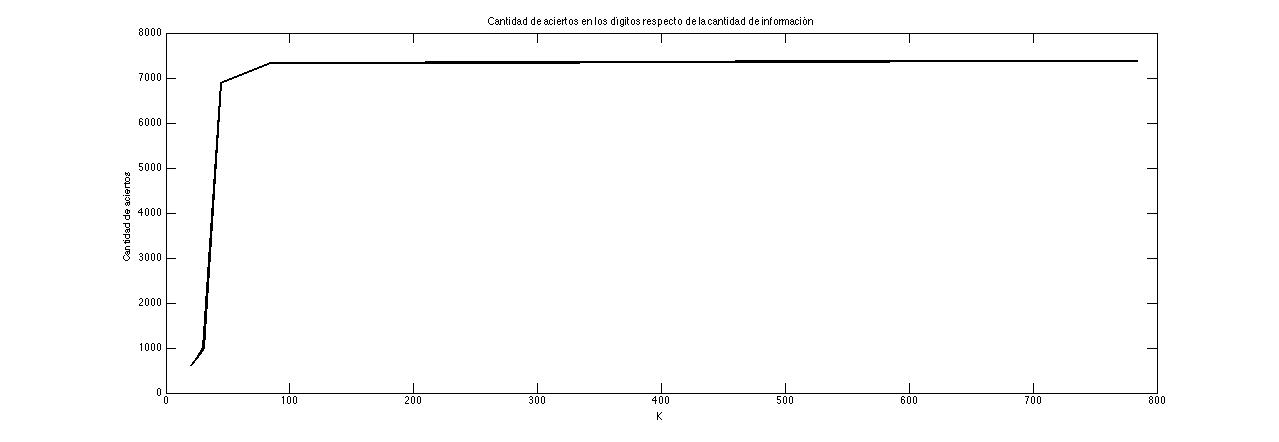
\includegraphics[width=540pt]{../imgs/aciertosconk.jpg}
\caption[h]{Cantidad de Aciertos respecto de K a partir de 10000 imágenes.}
\end{center}
\end{figure}

En el gráfico anterior puede observarse que, si bien los resultados son más precisos, alcanza con guardar el 6\% de los datos de cada imagen para alcanzar un 70\% de correctitud en la deducción de caracteres. Esto nos da lugar a pensar que, a pesar de ser mejor lograr una precisión del 73\%, no es realmente necesario almacenar toda la transformada característica de cada dí­gito para deducirlo. Sin embargo, decidimos otorgar la opción de procesar la matriz entera variando $k$, para que el procesamiento de la base de datos pueda realizarse como el usuario lo desea. 

\subsection{Detalles de Implementación}
Nuestro trabajo consistió en implementar las funciones mencionadas anteriormente. Para el desarrollo del mismo, diversas herramientas fueron necesarias. En esta sección, se explicita la utilización de las mismas aclarando en qué nos ayudaron a lograr una correcta ejecución de nuestra implementación.  
\subsubsection{Implementación en C}
En el caso de $C$, las implementaciones se realizaron siguiendo algoritmos sencillos. Para recorrer las matrices de píxeles utilizamos $for$ pues nos pareció lo más conveniente considerando que nuestros valores estaban pre-establecidos y que al colocar un for dentro de otro (uno para las filas y otro para las columnas) era más simple recorrer todas las posiciones de una matriz.

\newline
Por un lado utilizamos, como tipo de datos, los floats debido a que no nos resultó necesario un gran nivel de precisión para lograr los resultados deseados, evitandonos extender el código y su complejidad para utilizar doubles.

\newline
Luego, con el fin de disminuir el tiempo de ejecución de $C$, comprimimos partes del código reduciendo, a su vez, la cantidad de líneas. También, alteramos pequeños detalles que sumados marcarían diferencia. Por ejemplo, cambiamos j++ por ++j. De este modo, logramos optimizar el código lo máximo posible para hallar una justificación más profunda a la comparación de tiempo con $Assembler$. 

Nuestras funciones se realizaron del siguiente modo:

{\Large{\textit{\textsl{$CargarLabel$}}}:} \end{Large} Como bien lo indica su nombre, la función $cargarLabel$ se encarga de cargar las etiquetas que determinan qué dígito se encuentra en cada fila de la base de datos. Para esto, se utilizan las funciones $open$ y $close$ proporcionadas por $fstream$ para abrir $label.txt$. Finalmente, se almacena elemento a elemento en la matriz $label$ ingresada como parámetro a través de la función $set$. Dicha función es la que se utiliza en las funciones presentadas a continuación para almacenar valores en variables dentro del programa.\\

{\Large{\textit{\textsl{$CargarVt$}}}:} \end{Large}  Esta función abre el archivo $Vt.txt$ y se encarga de recorrerlo para almacenar su contenido en la matriz $Vt$ dentro de un ciclo. En el caso en el que el archivo sea inexistente, se abre el archivo $matriz.txt$ y se crea una matriz $base$ cuyos elementos son los de la matriz del archivo. Luego, se calcula $mediaCero$ de la matriz cargada y se la traspone. Posteriormente, se multiplica $base$ con su propia traspuesta y se divide el resultado obtenido $E$ por $n$-1, siendo $n$ la cantidad de filas de la matriz. Las matrices en cuestión son, más tarde, eliminadas. 
La función continúa aplicándole $algoritmoQR$ a $E$ y ubica el resultado en $V$ para luego eliminar $E$, trasponer $V$ y guardarla en $Vt.txt$.\\

{\Large{\textit{\textsl{$CargarTc$}}}:} \end{Large} Tal como lo indica su nombre, esta función se encarga de cargar la matriz $Tc$. Para esto, realiza el mismo procedimiento que efectúa $cargarVc$ a diferencia de que, cuando el archivo $TC.txt$ no existe, se lo genera trasponiendo la matriz contenida en $matriz.txt$, que es multiplicada por la matriz original, y se calcula la matriz promedio con label a través de la función $calcularPromedioTC$.\\

{\Large{\textit{\textsl{$CargarCaracter$}}}:} \end{Large} Esta función se encarga de abrir el archivo $digito.txt$ y simplemente cargar su contenido a una matriz $X$, para, finalmente, cerrarlo.\\

{\Large{\textit{\textsl{$Matriz\_create$}}}:} \end{Large} Para la realización de esta función, nos limitamos a pedir memoria para la estructura Matriz y para su vector correspondiente. A la memoria pedida para la estructura le asignamos los tamaños de filas y columnas correspondientes (ingresados como parámetros de entrada). Luego, para el vector de la matriz pedimos memoria de tamaño $\#filas^*\#columnas$, para luego asignar el puntero obtenido al campo vector de la estructura.\\

{\Large{\textit{\textsl{$Delete\_matriz$}}}:} \end{Large} En esta función, liberamos los punteros creados al generar la matriz. Para ello, aplicamos $delete$ del puntero del vector de la matriz ingresada por parámetro para luego aplicarle la misma función a la matriz original y liberar la memoria reservada para ella.\\

{\Large{\textit{\textsl{$Matriz\_cero$}}}:} \end{Large} La función $Matriz\_cero$ consiste en reemplazar los valores de la matriz ingresada por parámetro con ceros. Para ello, se recorre toda la matriz mediante dos $for$ anidados y mediante la función $set$ se le asigna un 0 a cada posición de la matriz.
 
\begin{center}
\textbf{Matriz de Ceros}
\[ \left( \begin{matrix}
                    1 & 2 & 3 \\
                    4 & 5 & 6 \\
                    7 & 8 & 9
\end{matrix} \right) \Rightarrow \left( \begin{matrix}
					0 & 0 & 0 \\
                    0 & 0 & 0 \\
                    0 & 0 & 0
 \end{matrix} \right) \]
\end{center}

{\Large{\textit{\textsl{$Identidad$}}}:} \end{Large} Esta función genera una matriz identidad a partir de una matriz ingresada por parámetro. Para esto, la recorre mediante dos $for$ anidados. Para cada valor, la función verifica si se encuentra en la diagonal de la matriz o no con un $if$. En el caso de pertenecer a la diagonal, se le asigna mediante la función $set$ un $1$. Caso contrario, se le asigna un $0$.

\begin{center}
\textbf{Matriz Identidad}
\[ \left( \begin{matrix}
                    1 & 2 & 3 \\
                    4 & 5 & 6 \\
                    7 & 8 & 9
\end{matrix} \right) \Rightarrow \left( \begin{matrix}
					1 & 0 & 0 \\
                    0 & 1 & 0 \\
                    0 & 0 & 1
 \end{matrix} \right) \]
\end{center}

{\Large{\textit{\textsl{$Multiplicar$}}}: } \end{Large} Esta función toma dos matrices $A \in \mathbb{R}^{nxm}$ y $B \in \mathbb{R}^{mxk}$ ingresadas como parámetro y las multiplica. En primer lugar, controla las dimensiones de las matrices, si la cantidad de columnas de la primera no coincide con la cantidad de filas de la segunda, muestra por pantalla un mensaje de error. Caso contrario, se crea una matriz $C \in \mathbb{R}^{nxk}$ a la cual se le asigna el valor $0$ a todos sus elementos mediante la función $cero$ ya que ésta va a ir almacenando los resultados parciales.

\newline
En el ciclo del programa se van calculando los valores de cada una de las posiciones de $C$ de la siguiente forma:
C$_{i,j}$ = $\sum_{r=1}^{m} A_{i,r} B_{r,j}$. Para esto, se implementaron 3 $for$ anidados que controlan los índices $i, j, r$. Dentro de éstos, se extraen mediante la función $get$ los valores de $A_{i,r}$ y $B_{r,j}$. Posteriormente, se los multiplica y se los suma al valor parcial almacenado en $C_{i,j}$. Este proceso se realiza hasta llegar al final de las matrices.

\begin{center}
\textbf{Multiplicación de Matrices}
\[
\begin{pmatrix}
                    1 & 2 & 3 \\
                    4 & 5 & 6 \\
                    7 & 8 & 9
\end{pmatrix} \times
\begin{pmatrix}
                    1 & 2 & 3 \\
                    4 & 5 & 6 \\
                    7 & 8 & 9
\end{pmatrix}
=
\begin{pmatrix}
                    30 & 36 & 42 \\
                    66 & 81 & 96 \\
                    102 & 126 & 150
\end{pmatrix}
\]
 
\end{center}\newline
{\Large{\textit{\textsl{$MultiplicarThis$}}}: } \end{Large} Esta función toma dos matrices $A \in \mathbb{R}^{nxn}$ y $B \in \mathbb{R}^{nxn}$ por parámetro y realiza $A = A * B$. Para esto, se utiliza la función $multiplicar$ la cual genera una matriz $C$ con el resultado de $A * B$. Posteriormente, se copia la matriz $C$ en $A$ mediante la función $copiar$. 

\begin{center}
\textbf{MultiplicarThis}
\[
A = \begin{pmatrix}
                    1 & 2 & 3 \\
                    4 & 5 & 6 \\
                    7 & 8 & 9
\end{pmatrix} \times B =
\begin{pmatrix}
                    1 & 2 & 3 \\
                    4 & 5 & 6 \\
                    7 & 8 & 9
\end{pmatrix} \Rightarrow
A =
\begin{pmatrix}
                    30 & 36 & 42 \\
                    66 & 81 & 96 \\
                    102 & 126 & 150
\end{pmatrix}
\]
 
\end{center}\newline

{\Large{\textit{\textsl{$MultiplicarParametro$}}}: } \end{Large} La función $multiplicarParametros$ toma dos matrices $A \in \mathbb{R}^{nxn}$ y $B \in \mathbb{R}^{nxn}$ por parámetro y realiza $B = A * B$. Para esto, se utiliza la función $multiplicar$ la cual genera una matriz $C$ con el resultado de $A * B$. Posteriormente, se copia la matriz $C$ en $B$ mediante la función $copiar$. En otras palabras, la función realiza el mismo procedimiento que $multiplicarThis$ a diferencia de que la matriz resultante se almacena en $B$ y no en $A$.
\begin{center}
\textbf{MultiplicarParámetro}
\[
A = \begin{pmatrix}
                    1 & 2 & 3 \\
                    4 & 5 & 6 \\
                    7 & 8 & 9
\end{pmatrix} \times B =
\begin{pmatrix}
                    1 & 2 & 3 \\
                    4 & 5 & 6 \\
                    7 & 8 & 9
\end{pmatrix} \Rightarrow
B =
\begin{pmatrix}
                    30 & 36 & 42 \\
                    66 & 81 & 96 \\
                    102 & 126 & 150
\end{pmatrix}
\]
 
\end{center}\newline
{\Large{\textit{\textsl{$Dividir$}}}: } \end{Large} Esta función toma una matriz $A$ y un float $v$ por parámetro y divide a todos los elementos de $A$ por $v$. Para esto, recorre toda la matriz mediante dos $for$ anidados y para cada $A_{i,j}$, obtenido mediante la función $get$, realiza $A_{i,j} / v$. Posteriormente, almacena este valor en la misma posición utilizando la función $set$.
\begin{center}
\textbf{División por 2}
\[ \left( \begin{matrix}
                    1 & 2 & 3 \\
                    4 & 5 & 6 \\
                    7 & 8 & 9
\end{matrix} \right) \Rightarrow \left( \begin{matrix}
					1/2 & 1 & 3/2 \\
                    4/2 & 5/2 & 3 \\
                    7/2 & 4 & 9/2
 \end{matrix} \right) \]
\end{center}\newline

{\Large{\textit{\textsl{$Copiar$}}}: } \end{Large}Esta función toma dos matrices $A \in \mathbb{R}^{nxm}$ y $B \in \mathbb{R}^{nxm}$ por parámetro y copia los elementos de $B$ en $A$. Para esto, recorre toda la matriz mediante dos $for$ anidados, toma $B_{i,j}$ mediante la función $get$ y lo coloca en $A_{i,j}$ utilizando la función $set$.\\

{\Large{\textit{\textsl{$Traspuesta$}}}: } \end{Large}Esta función toma dos matrices $A \in \mathbb{R}^{nxm}$ y $B \in \mathbb{R}^{mxn}$ por parámetro y traspone la matriz $A$ para luego almacenarla en $B$. Para esto, recorre toda la matriz mediante dos $for$ anidados y toma $A_{i,j}$ mediante la función $get$ y lo coloca en $B_{j,i}$ utilizando la función $set$. 

\begin{center}
\textbf{traspuesta}
\[ \left( \begin{matrix}
                    1 & 2 & 3 & 1\\
                    4 & 5 & 6 & 2\\
                    7 & 8 & 9 & 3
\end{matrix} \right) \Rightarrow \left( \begin{matrix}
					1 & 4 & 7 \\
                    2 & 5 & 8 \\
                    3 & 6 & 9 \\
                    1 & 2 & 3
 \end{matrix} \right) \]
\end{center}\newline

{\Large{\textit{\textsl{$TraspuestaCuadrada$}}}: } \end{Large} La función $traspuestaCuadrada$ toma una matriz $A \in \mathbb{R}^{nxn}$ y la traspone. Para esto, recorre los elementos de la matriz que se encuentran por encima de la diagonal mediante dos $for$ anidados. En cada iteración toma $A_{i,j}$ mediante la función $get$ y lo coloca en una variable auxiliar $aux1$. posteriormente, toma $A_{j,i}$ y lo coloca en una variable auxiliar $aux2$. Por último, almacena $aux2$ en $A_{i,j}$ y $aux1$ en $A_{j,i}$ mediante la función $set$.
\begin{center}
\textbf{traspuestaCuadrada}
\[ \left( \begin{matrix}
                    1 & 2 & 3\\
                    4 & 5 & 6\\
                    7 & 8 & 9
\end{matrix} \right) \Rightarrow \left( \begin{matrix}
					1 & 4 & 7 \\
                    2 & 5 & 8 \\
                    3 & 6 & 9
 \end{matrix} \right) \]
\end{center}\newline


{\Large{\textit{\textsl{$MediaCero$}}}: } \end{Large} Esta función toma una matriz $A \in \mathbb{R}^{nxm}$ y suma todas sus columnas para, de este modo, obtener un vector $B \in \mathbb{R}^{1xm}$. Posteriormente, divide cada elemento de este vector por $n$. Por último, a cada fila de $A$ le resta $B$.

\begin{center}
\textbf{MediaCero}
\[
\begin{pmatrix}
                    1 & 2 & 3 \\
                    4 & 5 & 6 \\
                    7 & 8 & 9
\end{pmatrix} \Rightarrow
\begin{pmatrix}
                    6 \ 
                    15 \ 
                    24
\end{pmatrix} \Rightarrow
\begin{pmatrix}
                    2 \ 
                    5 \ 
                    8
\end{pmatrix} \Rightarrow
\begin{pmatrix}
                    -1 & 1 & 2 \\
                    -1 & 0 & 1 \\
                    -1 & 0 & 1
\end{pmatrix} 
\]
 
\end{center}\newline

{\Large{\textit{\textsl{$Set$}}}: } \end{Large} La función $set$ toma una matriz $A \in \mathbb{R}^{nxm}$, una fila $i$, una columna $j$ y un float $v$ para luego asignarle el valor $v$ a $A_{i,j}$. Para esto, calcula la posición de memoria de $A_{i,j}$ a partir de la siguiente fórmula: $puntero\ a\ la\ matriz + i * m + j$. Luego, le asigna el valor $v$ a dicha posición.\\

{\Large{\textit{\textsl{$Get$}}}: } \end{Large} Esta función toma una matriz $A \in \mathbb{R}^{nxm}$, una fila $i$ y una columna $j$ y devuelve el valor $v$ de $A_{i,j}$. Para esto, calcula la posición de memoria de $A_{i,j}$ a partir de la siguiente fórmula: $puntero\ a\ la\ matriz + i * m + j$. Luego, retorna el valor $v$ de dicha posición.\\

{\Large{\textit{\textsl{$Norma2$}}}: } \end{Large} La función $norma2$ toma un vector $A \in \mathbb{R}^{nx1}$ y le calcula la norma2\footnote{Para un vector $\vec{x}$ = ($x_1,x_2,...,x_n)$ se define la norma$-p$ como: $| \vec x \|_p = \sqrt[p]{|x_1|^p+|x_2|^p+...+|x_n|^p}$}. Para esto, recorre todo el vector con un $for$ y obtiene los valores mediante la función $get$. Luego, eleva dichos valores al cuadrado y los suma. Por último, calcula la raíz cuadrada del resultado obtenido.\\

{\Large{\textit{\textsl{$AveriguarDigito$}}}: } \end{Large} Esta función toma una matriz $A \in \mathbb{R}^{nx10}$ con las transformadas características de todos los dígitos y un vector $B \in \mathbb{R}^{kx1}$ con la transformada característica del dígito que se desea averiguar. Lo primero que realiza es restarle a cada transformada de $A$ el vector $B$. Luego, calcula la norma2 de la resta mediante la función $norma2$. Por último, compara todas las normas y se queda con la más chica, que resulta ser el dígito ingresado.\\

{\Large{\textit{\textsl{$Rotacion$}}}: } \end{Large} La función $rotacion$ recibe una matriz $A \in \mathbb{R}^{mxm}$,  una matriz $B \in \mathbb{R}^{mxm}$ y dos enteros $i$, $j$. Su objetivo es realizar una Rotación de Givens\footnote{http://bit.ly/1lHPmKY} que coloque un $0$ en $A_{i,j}$. Para esto, se multiplica a la matriz $A$ y a la matriz $B$ por una matriz $C$ donde:\\

\sgn $C_{n,m}$ = 
   \begin{cases} 
      $\cfrac{A_{j,j}}{\sqrt{A_{j,j}^2 + A_{i,j}^2}}$  & \mbox{si $n = m = i$}  \\
      $\cfrac{A_{j,j}}{\sqrt{A_{j,j}^2 + A_{i,j}^2}}$  & \mbox{si $n = m = j$}  \\
      $\cfrac{-A_{i,j}}{\sqrt{A_{j,j}^2 + A_{i,j}^2}}$  & \mbox{si $n = i\ \land\ m = j$}  \\
      $\cfrac{A_{i,j}}{\sqrt{A_{j,j}^2 + A_{i,j}^2}}$  & \mbox{si $n = j\ \land\ m = i$}  \\
      1  & \mbox{si  $n = m = k\, \forall (k \neq i\ ||\  k \neq j)$}  \\ 
      0 & \mbox{caso contrario}
   \end{cases}

Como la función rotación es muy utilizada, decidimos optimizarla modificando únicamente las filas $i$ y $j$ en vez de multiplicar las matrices dado que el resto de las filas no varía.\\


{\Large{\textit{\textsl{$FactorizacionQR$}}}: } \end{Large} La factorización $QR$ se realiza con el método de Givens. La función encargada de realizar dicha factorización comienza aplicándole la función identidad a la matriz $Q$ ingresada por parámetro. Luego, realiza dos ciclos ($for$) para recorrer la matriz dentro de los que se evalúa si el valor absoluto del elemento ($i,j$) de la matriz $self$ es mayor o igual a la tolerancia ingresada por parámetro de entrada. En caso de ser así, se llama a la función $rotacion$ de $self$ y $Q$ en la posición en cuestión. Al finalizar de recorrer la matriz, se aplica $traspuestaCuadrada$ a la matriz $Q$.\\

{\Large{\textit{\textsl{$FactorizacionQR$}}}: } \end{Large} La factorización $QR$ se realiza con el método de Givens. La función encargada de realizar dicha factorización comienza aplicándole la función identidad a la matriz $Q$ ingresada por parámetro. Luego, realiza dos ciclos ($for$) para recorrer la matriz dentro de los que se evalúa si el valor absoluto del elemento ($i,j$) de la matriz $self$ es mayor o igual a la tolerancia ingresada por parámetro de entrada. En caso de ser así, se llama a la función $rotacion$ de $self$ y $Q$ en la posición en cuestión. Al finalizar de recorrer la matriz, se aplica $traspuestaCuadrada$ s la matriz $Q$.\\

{\Large{\textit{\textsl{$AlgoritmoQR$}}}: } \end{Large} $algoritmoQR$ crea las matrices $Qk$ y $Rk$ y le aplica la función identidad a la matriz $V$ ingresada como parámetro. Luego, se ejecuta un ciclo que le aplica $factorizacionQR$ a $self$ con $Qk$ y multiplica, por un lado, $self$ con $Qk$ y, por el otro, $V$ con $Qk$ siempre que no se llegue a la $paradaQR$ de $self$ con $toleranciaSumaSuperior$. Luego de dicho ciclo se eliminan las matrices $Qk$ y $Rk$.\\

{\Large{\textit{\textsl{$ParadaQR$}}}: } \end{Large} Esta función realiza la suma del valor absoluto del elemento ($i,j$) de la matriz $self$ ingresada como parámetro. Para ello, se recorre la matriz $self$ a partir de dos ciclos, uno dentro del otro. La función devuelve un booleano que indica si la tolerancia $tol$ ingresada como parámetro resulta mayor a la suma realizada.\\

{\Large{\textit{\textsl{$CalcularPromedioTC$}}}: } \end{Large} Esta función crea dos matrices, $Tc$ y $cantidad$, que inicializa en cero. Luego, se ejecuta un ciclo que inserta en $cantidad$ su valor inicial+1 y otro que realiza lo mismo con $Tc$ a diferencia de que le agrega el valor inicial+$self$. Por otro lado, se ejecuta un ciclo que obtiene cada posición de $Tc$ y la divide por el elemento correspondiente de $cantidad$, para luego reubicarlo en la matriz $Tc$. Finalmente elimina $cantidad$ y devuelve $Tc$.


\subsubsection{Implementación en Assembler}
Para la implementación en $Assembler$, utilizamos la extensión SSE para procesar varios bits a la vez. Esta herramienta nos permitió acelerar la ejecución de nuestro programa dado que en cada ciclo (en los casos en los que fue utilizado) se tratan 16 bytes a la vez.
Por otro lado, preferimos utilizar floats en vez de doubles pues, si bien la precisión es menor y puede generar pequeñas diferencias, las imágenes obtenidas resultaban tan límpidas como las obtenidas por el tipo de datos de mayor precisión. De esta manera, con el fin de simplificar nuestro código, preferimos no utilizar registros innecesariamente y evitar largos ciclos que disminuirían el tiempo de ejecución del programa.  

Nuestras funciones se realizaron del siguiente modo:

{\Large{\textit{\textsl{$Matriz\_create$}}}: } \end{Large} Para la realización de esta función, nos limitamos a pedir memoria con $malloc$ moviendo a $rdi$ el tamaño de una matriz (16 bytes\footnote{$int$ fila + $int$ columna + $puntero$ vector = 4 + 4 + 8}).
\newline
Luego, al puntero retornado por $rax$ le asignamos los tamaños de fila y columna correspondientes (ingresados como parámetro de entrada) al igual que el puntero al vector de la matriz. Para realizar las asignaciones mencionadas se utiliza $mov\ dword[rax+offset\_fila], valor\ fila\ o\ columna$ pues se trata de enteros (4 bytes), luego double words. Para el puntero al vector de la matriz, realizamos una nueva llamada a $malloc$ en la que el tamaño ingresado por $rdi$ es $\#filas^*\#columnas$. Este último puntero obtenido es asignado al $offset\_vector$ de la matriz con la operación $mov$ $qword[puntero$ $matriz + offset\_vector], rax$. Se realiza la asignación de un qword dado que el tamaño de un puntero es de 8 bytes.\newline


{\Large{\textit{\textsl{$Delete\_matriz$}}}: } \end{Large} En esta función, liberamos los punteros creados al generar la matriz. Para ello, llamamos a $free$ del puntero del vector de la matriz ingresada por parámetro para luego aplicarle la misma función a la matriz original y liberar la memoria reservada para ella, ambos procesos se realizan con $mov\ rdi,\ [rbx+offset\_vector]$ y $mov\ rdi,\ rbx$ respectivamente, siendo $rbx$ el puntero a la matriz.\newline


{\Large{\textit{\textsl{$Matriz\_cero$}}}: } \end{Large} La función $Matriz\_cero$ consiste en reemplazar los valores de la matriz ingresada por parámetro con ceros. Para ello, simplemente se recorre la matriz avanzando el puntero a ésta de a 4 bytes y, paso a paso, agregando una máscara de ceros en la posición apuntada por el puntero hasta llegar al final de la matriz, para esto, se realiza un $movups\ [rdi],\ xmm0$ donde $rdi$ contiene el puntero al vector de la matriz y $xmm0$ la máscara de ceros. Se utiliza $movups$ pues se mueven floats; pero dado que se trata de un registro conteniendo ceros, el tipo de datos no afecta el copiado. Para matrices que no son múltiplo de 4, la función retrocede las posiciones que se pasó para procesar los últimos 4 bytes, sea cual sea el valor con el que se pasa. Para esto último, realiza la operación $imul\ rax,\ 4$, para luego sumarle el resultado obtenido a $rdi$ (como el resultado obtenido es negativo, se resta la cantidad de bytes que se pasó) y posicionarse en los últimos bytes.\newline


{\Large{\textit{\textsl{$Matriz\_identidad$}}}: } \end{Large} Esta función genera una matriz identidad a partir de un puntero a una matriz ingresado por parámetro.

Para realizarla, implementamos el procedimiento que se encuentra a continuación:
\begin{enumerate}
\item Calculamos la cantidad de iteraciones a realizar dividiendo la cantidad de columnas por 4 con el fin de conocer la cantidad de veces que se van a aplicar las funciones de 128 bits. Los bits restantes se procesan separadamente. Para dicho cálculo, nos limitamos a multiplicar $\#filas^*\#columnas$ (con $mul$) y a dividir dicho resultado por 4 (con $shr\ eax,\ 2$, siendo $eax$ el registro conteniendo $\#filas^*\#columnas$).
\item Luego, guardamos las máscaras necesarias con la función $movups$ que mueve $floats$ para crear la matriz identidad en registros con el fin de no tener que realizar llamadas a memoria dentro del ciclo dado que aumentan el tiempo de ejecución. Dichas máscaras son:
\begin{itemize}
\item $UnoIdentidad$: $$1\ \ 0\ \ 0 \ \ 0$$
\item $DosIdentidad$: $$0\ \ 1\ \ 0\ \ 0$$
\item $TresIdentidad$: $$0\ \ 0\ \ 1\ \ 0$$
\item $CuatroIdentidad$: $$0\ \ 0\ \ 0\ \ 1$$
\end{itemize}

Luego, este procedimiento se realiza a través de funciones de este tipo:

\begin{verbatim}
              movups xmm1, [DosIdentidad]
\end{verbatim}

\item El ciclo del programa consiste en una comparación entre la cantidad de iteraciones con 0 utilizando $cmp\ eax,\ 0$, caso que indica el fin de la ejecución, y una comparación del registro $r11$ con 0 que indica si ya se puso el 1 en la fila en cuestión y que se debe rellenar la fila con ceros.
\begin{enumerate}
\item Si ya se puso el 1 en la fila, se ubica la máscara de ceros en la posición de memoria apuntada por el puntero con $movups$ por el motivo explicado anteriormente.
\item Si no se ubicó el 1, se indica con el registro $bl$ en qué posición debe ser ubicado. El registro $bl$ es incrementado en 1 con la función $inc$ cada vez que se agrega el uno en una fila, cuando dicho valor es el 3, se realiza un $xor\ bl,\ bl$ que lo resetea.
\end{enumerate}
\item En el caso en el que queden bits sin procesar, el programa compara la cantidad de elementos de las filas de la matriz con $\#columnas\ - (\#columnas\ 'mod'\ 4)$. 
Los bits restantes son procesados uno por uno a través de un ciclo que termina una vez que se llega al final de la fila en cuestión. Esto se realiza a través con el siguiente procedimiento:
\begin{verbatim}
.finFila:
                ;termina la fila, se verifica que haya quedado todo en 0
                cmp r8d, 0
                je .voyAlCiclo
                mov dword[r14], 0
                add r14, 4
                dec r8d
                jmp .finFila
\end{verbatim}
donde $r8$ es el contador columna y $r14$ posee el puntero al vector.
\end{enumerate}\newline


{\Large{\textit{\textsl{$matriz\_multiplicar$}}}: } \end{Large} Esta función, como bien lo indica su nombre, se encarga de multiplicar matrices. Para ello, procesa las matrices $A \in \mathbb{R}^{nxm}$ y $B \in \mathbb{R}^{mxk}$ ingresadas como parámetro y 
crea una matriz $C\ \in \mathbb{R}^{nxk}$ = $A^*B$. La función realiza los siguientes pasos:
\begin{enumerate}
\item Se calcula la posición en la que se deben levantar los datos en la matriz $B$, ésta está dada por el puntero a destino + tamaño del dato * $\#columnas$*$i$ + tamaño del dato*$j$. Este cálculo se realiza del siguiente modo:

\begin{verbatim}
                movdqu xmm9, xmm2 ; j3|j2|j1|j0
                movdqu xmm10, xmm9 ; xmm10 = j3|j2|j1|j0
                punpckldq xmm9, xmm4 ; xmm9 = j2|j0
                punpckhdq xmm10, xmm4 ; xmm10 = j3|j1
\end{verbatim}                
            
Se desempaquetan los datos con las funciones $punpckldq$ y $punpckhdq$ con el fin de obtener el espacio libre suficiente para poder multiplicarlos a posterior.

\begin{verbatim}
                psllq xmm9, 2 ; xmm9 = j2*tamDato|j0*tamDato
                psllq xmm10, 2 ; xmm10 = j3*tamDato|j1*tamDato
\end{verbatim}
Se multiplica $j$*tamaño del dato con $psllq$ pues consiste en una multiplicación por 4.

\begin{verbatim}
                ;tamaño del dato * #columnas * i              
                movdqu xmm7, xmm1 ; xmm7 = i3|i2|i1|i0
                movdqu xmm8, xmm1 ; xmm8 = i3|i2|i1|i0         
                shufps xmm8, xmm8, 39h ; xmm8 = i0|i3|i2|i1
\end{verbatim}
Se calcula el tamaño del dato * $\#columnas$ * $i$ con la función $shufps$ con el fin de obtener el siguiente resultado:
\begin{figure}[H] %[h] Aqui [b] para button [t] para top
\begin{center}
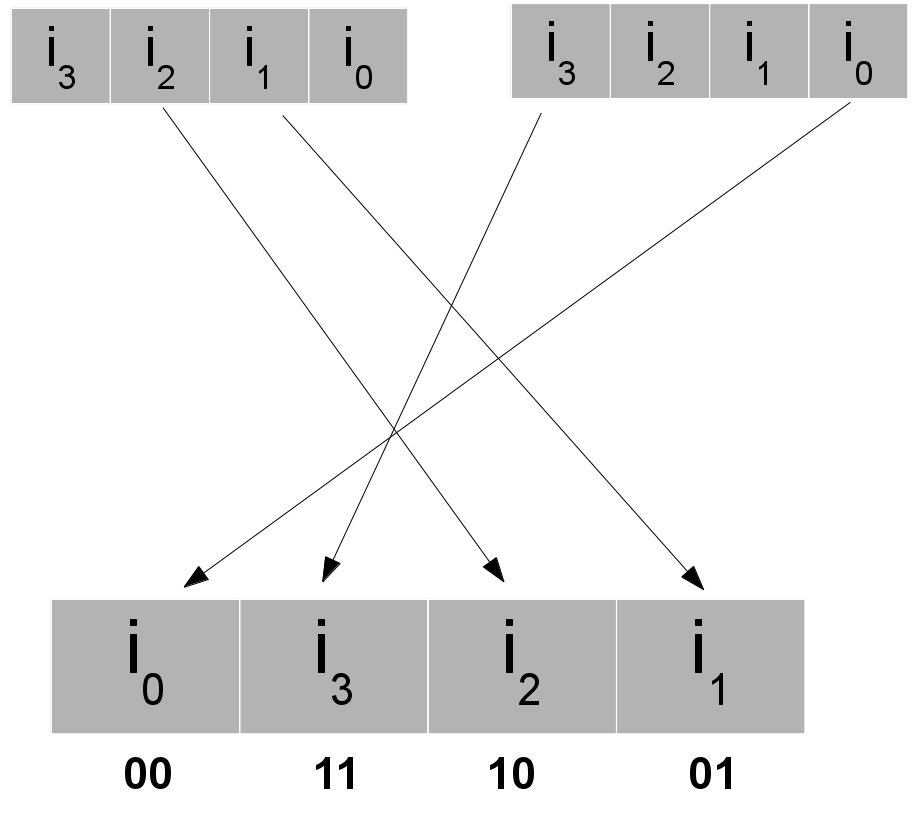
\includegraphics[width=120pt]{../imgs/arreglo1.jpg}
\end{center}
\end{figure}
\begin{verbatim}
                pmuludq xmm7, xmm5 ; xmm7 = i2*#columnas|i0*#columnas
                pmuludq xmm8, xmm5 ; xmm8 = i3*#columnas|i1*#columnas
\end{verbatim}
Se procede multiplicando $\#columas$ por las posiciones correspondientes con $pmuludq$, obteniendo como resultado $i_{2}$*$\#columnas$|$i_{0}$*$\#columnas$ y $i_{3}$*$\#columnas$|$i_{1}$*$\#columnas$.               
\begin{verbatim}            
                psllq xmm7, 2
                psllq xmm8, 2
               
                ;sumo dst + i + j
                paddq xmm7, xmm9
                paddq xmm8, xmm10
                paddq xmm7, xmm3 ; xmm7 = B2|B0
                paddq xmm8, xmm3 ; xmm8 = B3|B1
\end{verbatim}
Se shiftea el resultado obtenido a la izquierda con el fin de conseguir un registro con\\
 $i_{2}$*$\#columnas$*tamDato$|i_{0}$*$\#columnas$*tamDato y otro con \\\\
 $i_{3}$*$\#columnas$*$tamDato|i_{1}$*$\#columnas$*tamDato. Finalmente, se suma destino con $i$ y $j$ con $paddq$.

\item Se cargan los datos que serán multiplicados. Para esto se cargan los valores de $A$ y de $B$. Para cargar los de $A$ se copian simplemente los valores apuntados por el puntero con $movdqu$. Por otro lado, los valores de $B$ se extraen con la función $pextrq$ uno por uno para ser ubicados en su lugar correspondiente del siguiente modo:
\begin{verbatim}
                pextrq r9, xmm7, 1h ; r9 = B2
                movd xmm0, [r9] ; xmm0 = 0|0|0|B2
                xorps xmm10, xmm0 ; xmm10 = 0|0|B3|B2
                shufps xmm10, xmm10, 93h; xmm10 = 0|B3|B2|0
\end{verbatim}
Este procedimiento se realiza debido a que los valores a multiplicar se encuentran ubicados por columna entonces no pueden levantarse de a 4 en una única iteración y trasponer la matriz resulta temporalmente caro. Luego, se avanzan los punteros hasta haber recorrido enteramente las matrices.

\item Para procesar los últimos elementos en los casos en los que la matriz no tiene dimensión múltiplo de 4, se retroceden los últimos 4 elementos y se genera una máscara que contiene un 0 en las posiciones en las que la matriz ya fue procesada y un 1 en las otras, de este modo se filtran los datos para que éstos no sean procesados nuevamente. Para esto, se compara la cantidad de elementos procesados con la longitud de las columnas de la matriz en cuestión. Esto último se realiza de la siguiente manera:
\begin{verbatim}
                movd xmm12, r8d ; x|x|x|#columnas
                shufps xmm12, xmm12, 0h ; xmm12 = #columnas|#columnas|#columnas|#columnas
                pcmpgtd xmm12, xmm1 ; si i < #columnas pone 1's, sino 0's
                pand xmm12, xmm13 ; si i < #columnas pone 1, sino 0
                shufps xmm12, xmm12, 1Bh ; se acomoda la máscara (1|2|3|4 -> 4|3|2|1)
\end{verbatim}
Se compara el contador de columnas con la cantidad de columnas procesadas con $pcmgtd$ y se obtiene una máscara conteniendo ceros y unos que luego es filtrada con $pand$.
\begin{verbatim}
                ;modificación del índice de las filas
                movd xmm0, ecx ; x|x|x|contador
                shufps xmm0, xmm0, 0h
                paddd xmm1, xmm0 ; se le resta a i la cantidad de celdas que se pasó.
               
                imul rcx, 4 ;cantidad de bytes a retroceder            
                add r15, rcx ;retrocede A
\end{verbatim}
Estos pasos se realizan del mismo modo que $Matriz\_cero$, en donde se multiplican la cantidad de posiciones que se procesaron de más por cuatro para luego restarlas al puntero que apunta al vector y posicionarse correctamente para procesar los últimos datos.

\item Para guardar los datos en $C$, se realizan los siguientes pasos:
\begin{verbatim}
				;guardado de C
                movups xmm9, xmm11 ; xmm9 = suma3|suma2|suma1|suma0
                psrldq xmm9, 8 ;xmm9 = 0|0|suma3|suma2
                addps xmm11, xmm9  ; xmm11 = x|x|suma3+suma1|suma2+suma0
                movups xmm9, xmm11 ; xmm9 = x|x|suma3+suma1|suma2+suma0
                psrldq xmm9, 4 ; xmm9 = x|x|x|suma3+suma1
                addps xmm11, xmm9 ; xmm11 = x|x|x|sumatoria
                movd [r11], xmm11 ; guardado c
\end{verbatim}
Para realizar la sumatoria de los elementos almacenados en un registro $xmm$, se deben ubicar los elementos de la parte alta del registro en la parte baja de otro registro. Para esto, utilizamos $psrldq$ que shiftea a derecha elementos de tipo double quadword y pone ceros en el resto de las posiciones.
Luego, se utiliza $addps$ que se encarga de sumar registros de la siguiente forma:
\begin{figure}[H] %[h] Aqui [b] para button [t] para top
\begin{center}
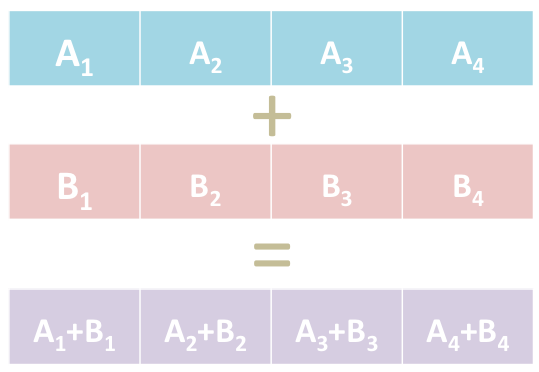
\includegraphics[width=160pt]{../imgs/registroSuma.jpg}
\end{center}
\end{figure}
Por último, se almacena la sumatoria obtenida en el espacio de memoria asignado por $r11$ con $movd$ pues se tratan de double words. 
\end{enumerate}\newline

{\Large{\textit{\textsl{$Matriz\_dividir$}}}: } \end{Large} La función $dividir$ calcula, en primer lugar, la cantidad de iteraciones a realizar multiplicando $\#filas$ por $\#columnas$ con el mismo procedimiento que se mencionó en las funciones anteriores. El ciclo principal de la función se encarga de levantar los datos apuntados por el puntero del vector con la función $movdqu$ y almacenarlos en un registro $xmm$. Luego, los divide por el valor ingresado por $rsi$ con la función $divps$ pues se trata de tipos de datos $floats$, para luego reemplazar los valores de la matriz original con
\begin{verbatim}
                movdqu [rdi], xmm1
\end{verbatim}

Para las matrices cuyas dimensiones no son múltiplo de 4, se realiza el procedimiento mencionado en la función anterior.\newline


{\Large{\textit{\textsl{$Matriz\_copiar$}}}: } \end{Large} La función $copiar$ simplemente efectúa la copia del contenido de una matriz a la otra del mismo modo que en la función $dividir$ a diferencia de que no se dividen los elementos y que éstos se copian en un vector destino y no en el fuente. Para esto se mueven los valores de la matriz fuente con $movdqu$ a la posición apuntada por el puntero destino dentro de un ciclo hasta el fin de la matriz del siguiente modo:
\begin{verbatim}
                movdqu xmm1, [rdi]
                movdqu [rsi], xmm1
\end{verbatim}
siendo $rdi$ el registro fuente y $rsi$ el registro destino.\newline


{\Large{\textit{\textsl{$Matriz\_traspuesta$}}}: } \end{Large} Para trasponer la matriz ingresada como parámetro, $traspuesta$ procesa sus datos de una forma similar a $multiplicar$. Esto significa que levanta los datos y realiza el cálculo de puntero a destino + tamaño del dato * $\#columnas$*$i$ + tamaño del dato*$j$ para saber en qué posición ubicarlos. Esto se realiza del siguiente modo:

\begin{verbatim}
                movdqu xmm9, xmm2
                shufps xmm9, xmm9, 0xD8 ; xmm9 = j3|j1|j2|j0           
                movdqu xmm10, xmm9 ; xmm10 = j3|j1|j2|j0
\end{verbatim}
En primer lugar, se realiza una mezcla de los elementos del registro de esta forma:
\begin{figure}[H] %[h] Aqui [b] para button [t] para top
\begin{center}
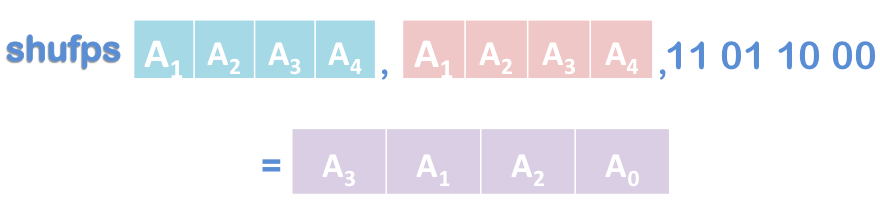
\includegraphics[width=250pt]{../imgs/sufps.jpg}
\end{center}
\end{figure}
Esto se debe a que, de este modo, los cálculos futuros se simplifican.
\begin{verbatim}           
                punpckldq xmm9, xmm4 ; xmm9 = j2|j0
                punpckhdq xmm10, xmm4 ; xmm10 = j3|j1

                psllq xmm9, 2 ; xmm9 = j2*tamDato|j0*tamDato
                psllq xmm10, 2 ; xmm10 = j3*tamDato|j1*tamDato
\end{verbatim}
Se procede desempaquetando el registro mezclado con $punpckldq$ para la parte baja y $punpckhdq$ para la parte alta. De este modo, se puede realizar una multiplicación con $psllq$ sin pérdida de precisión. De este modo, se obtiene $xmm9\ =\ j_2*tamDato|j_0*tamDato$ y $xmm10\ =\ j_3*tamDato|j_1*tamDato$.
\begin{verbatim}

                ;tamaño del dato * \#columnas * i              
                movdqu xmm7, xmm1 ; xmm7 = i3|i2|i1|i0
                movdqu xmm8, xmm1 ; xmm8 = i3|i2|i1|i0         
                shufps xmm8, xmm8, 39h ; xmm8 = i0|i3|i2|i1
                pmuludq xmm7, xmm15 ; xmm7 = i2*#columnas|i0*\#columnas
                pmuludq xmm8, xmm15 ; xmm8 = i3*#columnas|i1*\#columnas
               
                psllq xmm7, 2 ; xmm7 = i2*#columnas*tamDato|i0*\#columnas*tamDato
                psllq xmm8, 2 ; xmm8 = i3*#columnas*tamDato|i1*\#columnas*tamDato
\end{verbatim}
En el código anterior, se puede observar que se repite el procedimiento descrito anteriormente a diferencia de que se procesa el $tamaño\ del\ dato * \#columnas * i$. Para esto, se utilizan las mismas operaciones.
\begin{verbatim}              
                ;suma dst + i + j
                paddq xmm7, xmm9
                paddq xmm8, xmm10
                paddq xmm7, xmm3 ; xmm7 = dst2|dst0
                paddq xmm8, xmm3 ; xmm8 = dst3|dst1
\end{verbatim}
Luego, se realiza la suma del destino con $i$ y $j$. Para esto, se utiliza la función $paddq$ que suma los valores de los registros respetando las posiciones de cada uno de ellos.

Una vez dicha posición calculada, los elementos son ubicados uno a uno con $mov$ respectivamente luego de ser extraídos con $pextrq$ de la siguiente forma:
\begin{verbatim}
                pextrq rbx, xmm8, 1 ; rbx = dst3
                pextrd ecx, xmm0, 3 ; rcx = dato3
                mov dword [rbx], ecx
\end{verbatim}

Dado que los datos son double words, se utiliza $pextrd$ para extraerlos de la matriz original e insertarlos en un registro. Por otro lado, como los valores en $xmm8$ habían sido previamente desempaquetados, se utiliza $pextrq$ para extraerlos pues éstos son de tamaño quadword.

En el caso en el que la dimensión de la matriz no sea múltiplo de 4, los últimos elementos que no pueden ser procesados todos juntos se copian uno a uno de la misma manera a diferencia de que no se retrocede el puntero de la matriz fuente sino que se calcula la cantidad de elementos que restan procesar comparando los datos procesados con la cantidad de datos por fila. Esto último se realiza del siguiente modo:
\begin{verbatim}
                imul rax, 4 ;cantidad de bytes a retroceder            
                add r15, rax
\end{verbatim}
A partir de la multiplicación de $rax$ y de la suma a $r15$, el puntero es desplazado a la posición a partir de la cual se deben procesar los últimos bytes correctamente para que no se procesen elementos fuera de la matriz.\newline


{\Large{\textit{\textsl{$Matriz\_traspuestaCuadrada$}}}: } \end{Large} Esta función realiza el mismo procedimiento que la función anterior a diferencia de que la matriz fuente y destino son la misma dado que ambas poseen las mismas dimensiones. Luego, si bien el procedimiento es el mismo que el descrito anteriormente, con el fin de no perder datos al copiar los elementos a trasponer, los datos de las posiciones a ser reemplazadas son copiadas en dos registros e intercambiadas entre ellas del siguiente modo:
\begin{verbatim}
                pextrq rbx, xmm7, 0 ; rbx = dst0
                pextrq rcx, xmm11, 0 ; rcx = src0
                mov r15d, dword[rbx] ; r15 = dato dst0
                mov r14d, dword[rcx] ; r14 = dato src0
                mov dword[rbx], r14d
                mov dword[rcx], r15d
\end{verbatim}
Como puede observarse, se utilizan continuamente los registros $rbx$ y $rcx$, registros de fuente y de destino. De este modo, se realiza el copiado de una matriz a la otra en cada iteración en la que se procesan los elementos correspondientes.
 La paralelización en esta función se realiza al calcular la ubicación en la que deben agregarse los datos apuntados por el puntero fuente de esta forma:
 \begin{verbatim}
                cmp eax, 0
                je .fin ;si rax es 0 significa que terminó           
                mov r12d, 5
                paddd xmm1, xmm6 ; i3+4|i2+4|i1+4|i0+4 avanzo 4 filas
 \end{verbatim}
 Para avanzar, se utiliza $paddd$ en un registro $xmm$ con el fin de paralelizar operaciones y reducir iteraciones.\newline


{\Large{\textit{\textsl{$Matriz\_mediaCero$}}}: } \end{Large} En esta función, se comienzan sumando las filas de la matriz ingresada como parámetro en un vector, para esto se realiza lo siguiente:

\begin{verbatim}
                mov eax, r13d ; eax = #columnas
                mul ecx ; eax = #columnas * contador de filas
                shl rax, 2 ; rax = #columnas * contador de filas * tam del dato

                mov r12, rbx ; r12 = contador de columnas
                shl r12, 2 ; r12 = contador de columnas * tamaño del dato

                add r12, r15
                add r12, rax ; r12 = me posiciona en cont. fila, cont. columna de self
\end{verbatim}
En esta sección, se calculan la cantidad de iteraciones a realiza y se setean los contadores que permiten un correcto desplazamiento dentro de la matriz. Las funciones que se utilizan son las básicas necesarias para elementos de 32 bits como $add$, $shl$ y $mov$. Las operaciones que se realizan son las mismas que se describieron anteriormente.
Para las sumas, se realiza el siguiente procedimiento:
\begin{verbatim}
                movdqu xmm1, [r12] ; xmm1 = A3|A2|A1|A0
                mulps xmm1, xmm12 ; xmm1 = A3*flag|A2*flag|A1*flag|A0*flag
                addps xmm0, xmm1 ; xmm0 = suma3|suma2|suma1|suma0
\end{verbatim}
Se utilizan $mulps$ y $addps$ pues trata de operaciones entre elementos de tipo float .
Luego, se dividen dichas sumas por la cantidad de filas. Esto se realiza de la siguiente forma:
\begin{verbatim}
                divps xmm0, xmm2 
\end{verbatim}
De este modo, se obtiene $suma_3/\#filas|suma_2/\#filas|suma_1/\#filas|suma_0/\#filas$.
Por último, se le resta a cada fila de la matriz obtenida el vector obtenido utilizando $subps$ como se ve a continuación:
\begin{verbatim}
                subps xmm1, xmm0
\end{verbatim}
De este modo, se obtiene $resta_3|resta_2|resta_1|resta_0$. Para dicha resta, se recorre la matriz del mismo modo que para la suma hasta llegar al final de la misma.\newline


{\Large{\textit{\textsl{$Matriz\_norma2$}}}: } \end{Large} Para realizar la norma de la matriz obtenida por parámetro, se levantan 4 elementos con $movdqu$ y se los multiplica con $mulps$ por sí mismos de forma a obtener los elementos al cuadrado como se puede ver a continuación:
\begin{verbatim}
                movups xmm1, [rdi] ; e|e|e|e
                mulps xmm1, xmm1 ; e^2|e^2|e^2|e^2
\end{verbatim}

 Luego, se los suma con $addps$ del siguiente modo:
\begin{verbatim}
                addps xmm2, xmm1
\end{verbatim} 
con el fin de obtener el resultado $suma|suma|suma|suma$. 
Luego, se suman todos los elementos paulatinamente del siguiente modo:
\begin{verbatim}
                movups xmm1, xmm2 ; xmm1 = x|x|suma0+suma2|suma1+suma3
                psrldq xmm1, 4 ; xmm1 = x|x|x|suma0+suma2
                addps xmm2, xmm1 ; xmm2 = x|x|x|sumatoria
\end{verbatim}
Se utilizan funciones para floats a diferencia de $psrldq$ pues se desea shiftear de 4 posiciones.

Este ciclo se repite hasta el final de la matriz para finalmente aplicar la raíz de la suma obtenida con $sqrtpd$.\newline


{\Large{\textit{\textsl{$Matriz\_rotacion$}}}: } \end{Large} En esta función ingresa por parámetro una matriz $A \in \mathbb{R}^{mxm}$, una matriz $B \in \mathbb{R}^{mxm}$ y dos enteros $i$, $j$. Su objetivo es realizar una rotación de Givens que coloque un $0$ en $A_{i,j}$. Para esto, se comienza calculando las posiciones de memoria del comienzo de las filas $i$ y $j$ tanto de la matriz $A$ como de la matriz $B$ de la siguiente forma:
\begin{verbatim}

                ;puntero a matriz + tamaño del dato * #columnas * j
                mov eax, r13d ; eax = #columnas
                mul ecx ; rax = #columnas * j
                shl rax, 2 ; rax = #columnas * j * tamaño del dato

                mov r10, rax ; r10 = #columnas * j * tamaño del dato
                mov r8, rax ; r8 = #columnas * j * tamaño del dato
                add r10, r15 ; r10 = jk para self
                add r8 , r14 ; r8 = jk para Q
\end{verbatim}
En este conjunto de operaciones, se calcula la posición de memoria de $j_k$ para las matrices $self$ y $Q$. Para esto, se utilizan el puntero a la matriz, el tamaño de los daots, la cantidad de columnas y $j$. En primer lugar, se multiplican la cantidad de columnas con $j$, para esto se utiliza $mul$ pues consiste en una simple multiplicación de enteros. Luego, para multiplicar por la cantidad de datos, se realiza un $shl$ pues consiste en una multiplicación por 4 (se trata de floats). Por último, se suman los punteros a las matrices con el fin de contener en $r8$ la posición para $Q$ y en $r10$ la deseada para $self$.

Los cálculos que se realizan para las posiciones $i_k$, $x_1$ y $x_2$ siguen la misma estructura por lo que decidimos no realizar una descripción detallada de éstas.

Posteriormente, se calculan el $seno$ ($\cfrac{A_{i,j}}{\sqrt{A_{j,j}^2 + A_{i,j}^2}}$) y el $coseno$ ($\cfrac{A_j,j}{\sqrt{A_{j,j}^2 + A_{i,j}^2}}$) utilizando las siguientes operaciones:


\begin{verbatim}
                movups xmm1, xmm0 ; xmm1 = 0|0|x1|x2

                mulps xmm0, xmm1 ; xmm0 = x|x|x1²|x2²
                movups xmm2, xmm0 ; xmm2 = x|x|x1²|x2²
\end{verbatim}
Para la multiplicación de los elementos por ellos mismos, utilizamos $mulps$ de dos registros con el mismo contenido. Esto se debe a que esta operación consiste en una multiplicación de floats en un registro de 128 bits.
\begin{verbatim}
                psrldq xmm2, 4 ;xmm2 = 0|0|0|x1²

                addps xmm0, xmm2 ; xmm0 = x|x|x|x1²+x2²

                sqrtps xmm0, xmm0 ; xmm0 = x|x|x|sqrt(x1²+x2²)
\end{verbatim}
Luego, desplazamos el contenido de uno de los registros utilizados previamente de forma tal a obtener el valor $x_1$² en los últimos 32 bits para, luego, sumarlo con $x_2$
² utilizando $addps$. Finalmente, se aplica la raíz a dicho resultado con la función $sqrtps$, de este modo se obtiene $x|x|x|sqrt(x_1^2+x_2^2)$.

\begin{verbatim}
                shufps xmm0, xmm0, 0h
                divps xmm1, xmm0 ; xmm1 = 0|0|coseno|seno
\end{verbatim}
Más tarde, se realiza el cálculo del $seno$ y $coseno$. Para esto, se divide el registro contenedor de los valores originales de x por el registro que posee las raíces de las sumas explicitadas anteriormente.
\begin{verbatim}
                pextrd r12d, xmm1, 0 ; r12 = seno
                movd xmm0, r12d ; xmm0 = x|x|x|seno
                shufps xmm0, xmm0, 0h ; xmm0 = seno|seno|seno|seno

                pextrd r12d, xmm1, 1 ; r12 = coseno
                movd xmm1, r12d ; xmm1 = x|x|x|coseno
                shufps xmm1, xmm1, 0h ; xmm1 = coseno|coseno|coseno|coseno
\end{verbatim}

Finalmente, se replican los resultados obtenidos 4 veces dentro de cada registro de 128 bits mediante la función $shufps$. De esta forma, se obtiene un registro $xmm0$ conteniendo los valores de $seno$ y otro $xmm1$ conteniendo los valores de $coseno$.

Una vez en el ciclo principal del programa, se levantan 4 valores de la fila $i$ y 4 de la fila $j$, tanto de la matriz $A$ como de la matriz $B$. Para esto se utiliza simplemente la función $movups$.

Posteriormente, se calculan las siguientes funciones para ambas matrices:
\begin{itemize}
\item $aux1$ = ($coseno$ * $j_k$) + ($seno$ * $i_k$) la cual posteriormente se almacena en la posición $j_k$ de las matrices
\item $aux2$ = ($coseno$ * $i_k$) - ($seno$ * $j_k$) la cual posteriormente se almacena en la posición $i_k$ de las matrices
\end{itemize}
en donde $j_k$ representa al elemento de la fila $j$ e $ik$ al de la fila $i$. 
Para esto, se aplican las siguientes operaciones:
\begin{verbatim}
                mulps xmm2, xmm1 
                mulps xmm3, xmm0
                addps xmm2, xmm3
\end{verbatim}
Éstas se repiten para cada operación mencionada, adecuándose a la necesidad de cada paso.

Por último, se mueven 4 bytes los puntero de las filas $i$ y $j$ con la función $add$ aplicada a los punteros almacenados. \newline
En el caso de que la cantidad de columnas de las matrices no sea múltiplo de 4, se calcula cuántos floats falta procesar y se retrocede todos los punteros esa cantidad, al igual que en las funciones anteriores. Una vez hecho esto, se calculan los correspondientes $aux1$ y $aux2$. Por último, se extraen de a uno con $pextrd$ los valores que restaban procesar de $aux1$ y $aux2$ y se los almacena en sus posiciones correspondientes dentro de la matriz.
\section{Uso del programa}

Una vez descomprimido el archivo $Izcovich\ -\ Vita.tar.gz$, es necesario abrir $TP\_Final.pro$ en QtCreator. Una vez que se ejecuta el programa, se debe abrir el achivo $Makefile$ y deben modificarse las siguientes lineas:\newline
- En primer lugar, se debe borrar la linea $matriz\_asm.o$:
							$$(CC)\ -c\ (CFLAGS)\ (INCPATH)\ -o\ ``@''\ ``<''$$
- Luego, debe agregarse la linea:\newline
					   $matriz\_asm.o$:
							$$nasm\ -f\ elf64\ -g\ -F\ dwarf\ -o\ matriz\_asm.o\ codigo/matriz\_asm.asm$$
y el programa debe ser nuevamente ejecutado. Luego, puede utilizarse el ejecutable generado.

Dentro de la carpeta descomprimida, se van a encontrar ciertos archivos y tres carpetas. Dentro de la carpeta ``código'' se encuentran los archivos $.asm$, $.h$ y $.cpp$. En la carpeta ``archivos'' se ubica la matriz almacenada en un $.txt$ al igual que las etiquetas de cada dígito ``label.txt''. También, se encuentran en dicha carpeta los archivos en los que se almacenan las matrices $Vt$ y $Tc$ necesarias para el procesamiento de la matriz ingresada. Por otro lado, se halla la carpeta ``imagenes'' en donde se guardan las imágenes de los dígitos que se quiere determinar en archivos de tipo $JPG$. 

Para la utilización de nuestro programa, se debe abrir el archivo ejecutable $TP\_Final$ que se encuentra en la carpeta ``codigo''. Una vez ingresado al panel principal, deben seleccionarse los parámetros de acuerdo a lo que se desee realizar. En primer lugar, al utilizar el programa por primera vez, debe procesarse la base de datos. Para esto, debe existir el archivo ``matriz.txt'' mencionado anteriormente. En nuestro caso, este archivo consiste en una matriz de tipo int de tamaño 60000*784, en donde cada fila se corresponde con una imagen de 28*28. Para realizar el procesamiento, se debe elegir el lenguaje de programación que se desee utilizar, éstos son $C$ o $ASM$. Una vez seleccionada la opción, debe elegirse la cantidad de imágenes de la matriz que se desea tratar (en nuestro caso, un valor entre 1 y 60000). Por otro lado, debe ingresarse el tamaño de las imágenes que en nuestro caso es de 28*28 y, por último, la precisión con la que se quiere operar. Ésta consiste en un valor $k$ entre 0 y $cantidad\_de\_filas$*$cantidad\_de\_columnas$. Como se puede observar en la $Figura\ 1$, a partir de $k$ = 47 la precisión no altera significativamente el resultado. Una vez ingresados los parámetros, se debe ``Aceptar''. Por último, debe cargarse la imagen del dígito que se quiera averiguar y presionar ``Procesar''. Una vez que se calcule el resultado, el mismo será mostrado en la pantalla final.  

\section{Resultados}
A partir de los valores obtenidos luego de varias pruebas realizadas para calcular la cantidad de ejecuciones de cada función $C$ y $Assembler$, podemos concluir que cuanto mayor es el tamaño de la imagen a procesar, mayor es la cantidad de ciclos realizados por el programa como también el tiempo para procesarlos. Esto resulta lógico considerando que a mayor tamaño de imagen, más importante va a ser la cantidad de datos a procesar lo que implica que el tiempo de ejecución del programa sea más elevado.\newline
Luego de dichas conclusiones, decidimos utilizar objdump para lograr dar una explicación a lo obtenido:\newline

En primera instancia, hallamos que la cantidad de ciclos realizados por $Assembler$ es muy menor a la realizada por $C$. Esto se debe a que el $Assembler$ de $C$ realiza múltiples llamados a memoria en cada ciclo. Por ejemplo, la mayoría de los datos que utiliza son almacenados en la pila por lo que en cada iteración realiza operaciones utilizando, por ejemplo, [rbp-0x28]. Ésta es la causa principal del retraso temporal generado por el $C$ respecto del $Assembler$.\newline 

Por otra parte, hallamos que los códigos en $Assembler$ generados por los $C$ realizan operaciones innecesarias, como por ejemplo multiplicar por 1, dado que se producen de manera automática.\newline

Por último, encontramos que el ensamblado del $C$ no utiliza instrucciones SIMD, empaquetando y desempaquetando, por lo que la cantidad de operaciones a realizar está multiplicada por 16.\newline

\begin{figure}[H] %[h] Aqui [b] para button [t] para top
\begin{center}
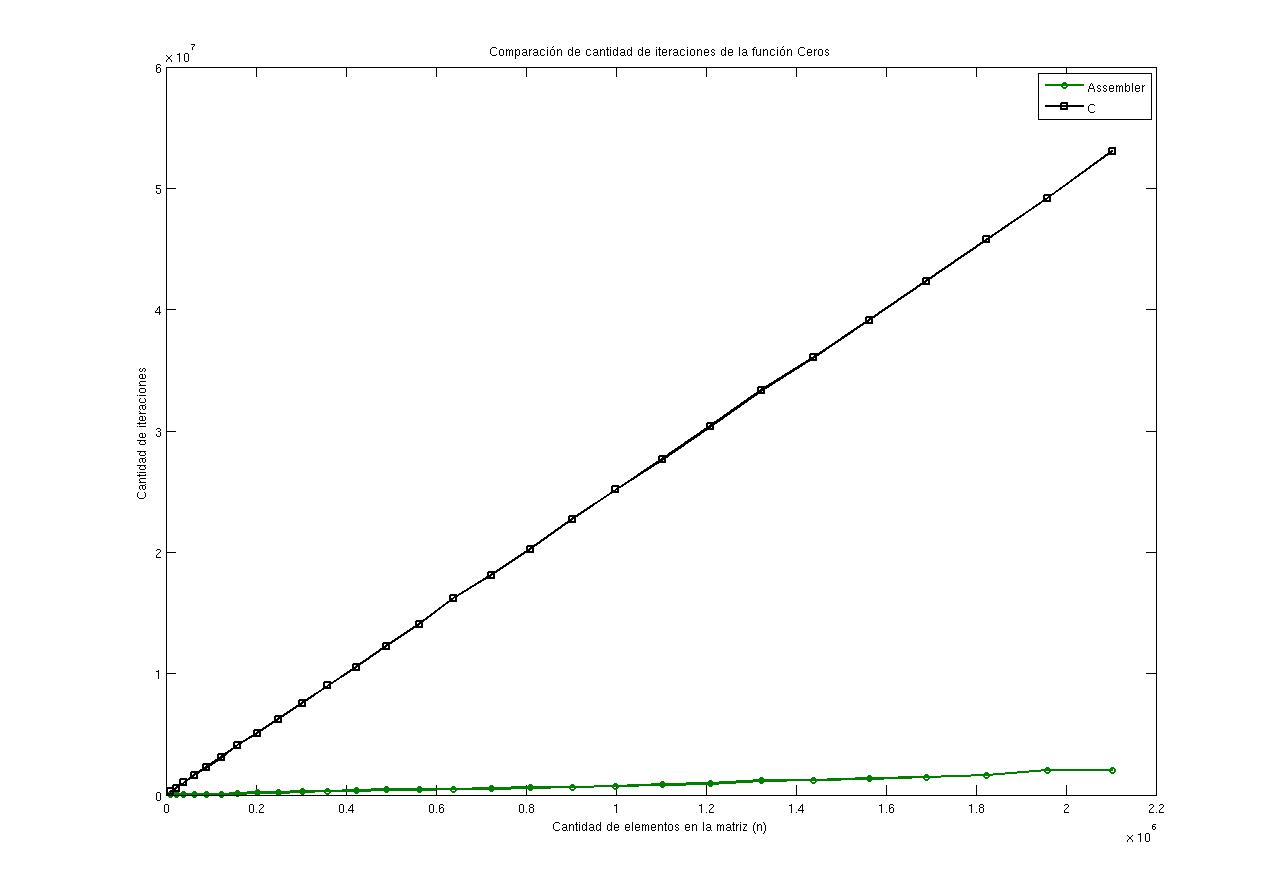
\includegraphics[width=500pt]{../imgs/comparacion_ceros.jpg}
\end{center}
\end{figure}

En el gráfico anterior, puede observarse que la función $Cero$ en $C$ utiliza una mayor cantidad de ciclos para ser procesada que $Matriz\_cero$ en $Assembler$. Esto se debe a que la función realizada en $C$ se encarga de reemplazar cada valor $(i,j)$ de la matriz original por un 0 a través de dos $for$, uno dentro del otro. Por otro lado, la función realizada en $Assembler$ realiza el mismo procedimiento a diferencia de que en vez de procesar una posición a la vez procesa cuatro. 
Al desensamblar el código de la función en $C$, notamos que la función realiza tres $call$ a distintas posiciones de memoria. Dado que para esto se accede a memoria, la función requiere más ciclos y tiempo para ejecutarse que la función que realizamos en $Assembler$ que no posee ninguno.

\begin{figure}[H] %[h] Aqui [b] para button [t] para top
\begin{center}
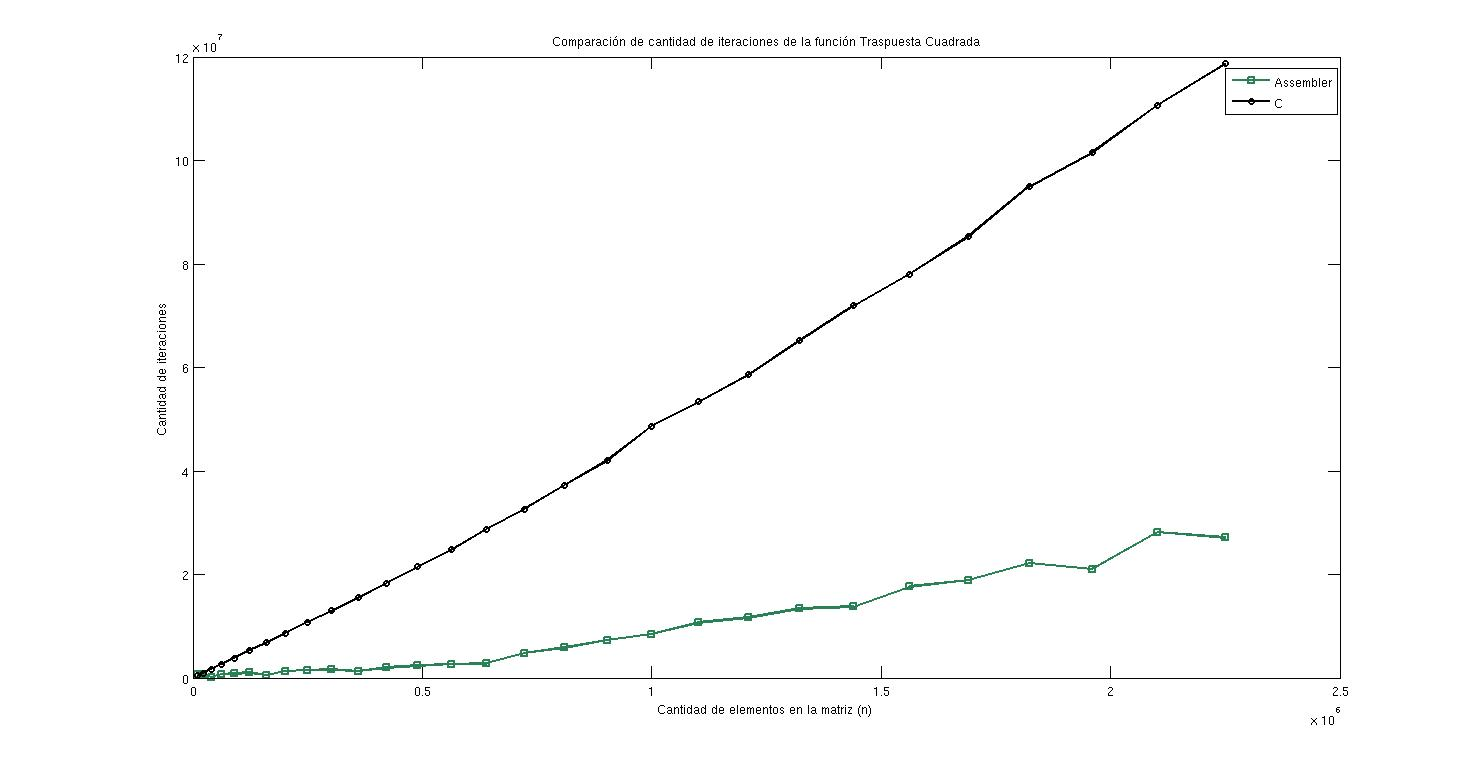
\includegraphics[width=500pt]{../imgs/comparacion_traspuestaCuadrada.jpg}
\end{center}
\end{figure}

\begin{figure}[H] %[h] Aqui [b] para button [t] para top
\begin{center}
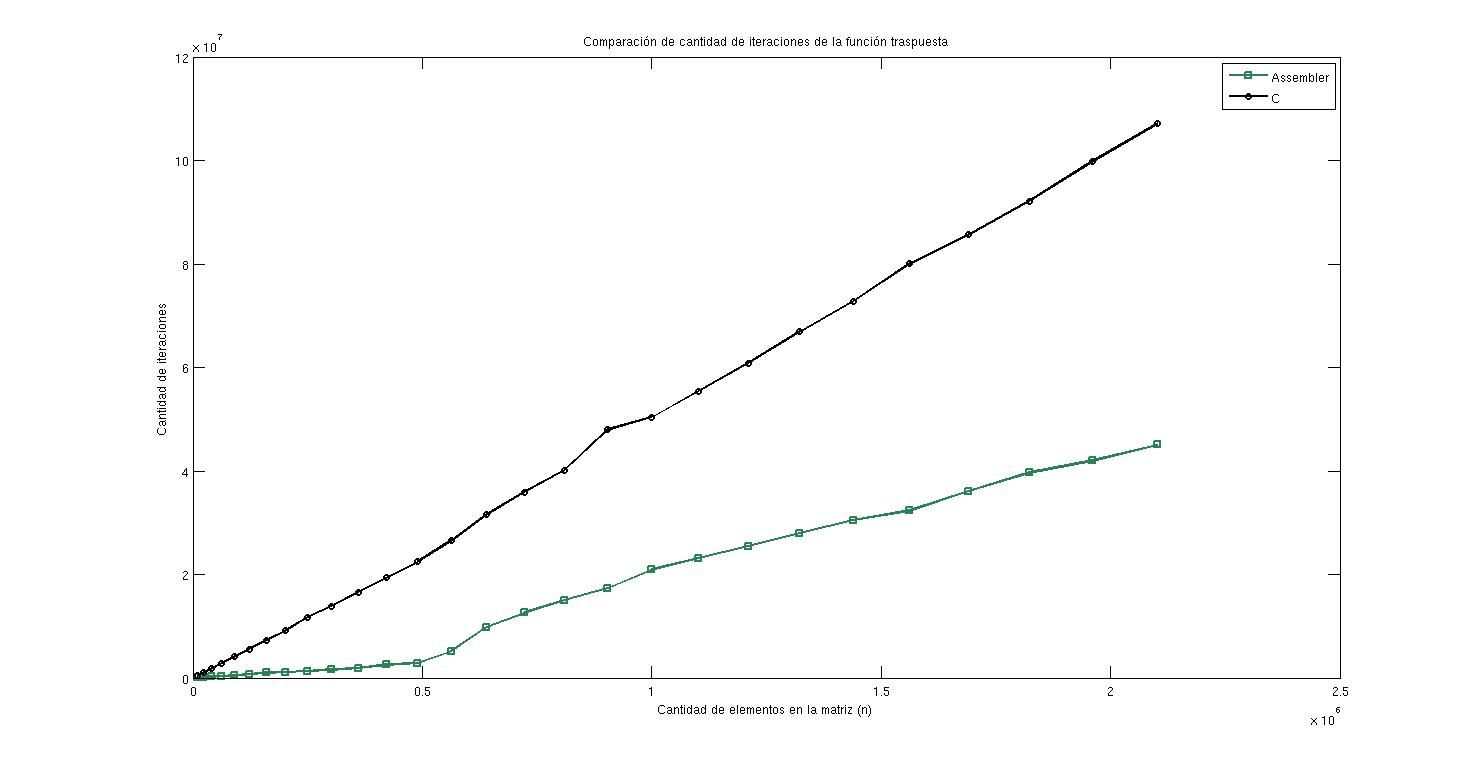
\includegraphics[width=500pt]{../imgs/comparacion_traspuesta.jpg}
\end{center}
\end{figure}

Los dos gráficos anteriores reflejan una gran diferencia respecto a la cantidad de iteraciones que realizan las mismas funciones en $C$ y en $Assembler$. Por un lado, puede verse al desensamblar el código que en ambas funciones se almacenan los valores en la pila con lo cual la función accede constantemente a ella utilizando $mov$ de la posición apuntada por $rbp$ y $rsp$. Dado que en la función realizada en $Assembler$ los valores se procesan a medida que son levantandos de la matriz original a través de registros de 128 bits y se almacenan directamente en la matriz destino, se evitan los almacenamientos y accesos a memoria constantes, que demoran la ejecución del código.  


\begin{figure}[H] %[h] Aqui [b] para button [t] para top
\begin{center}
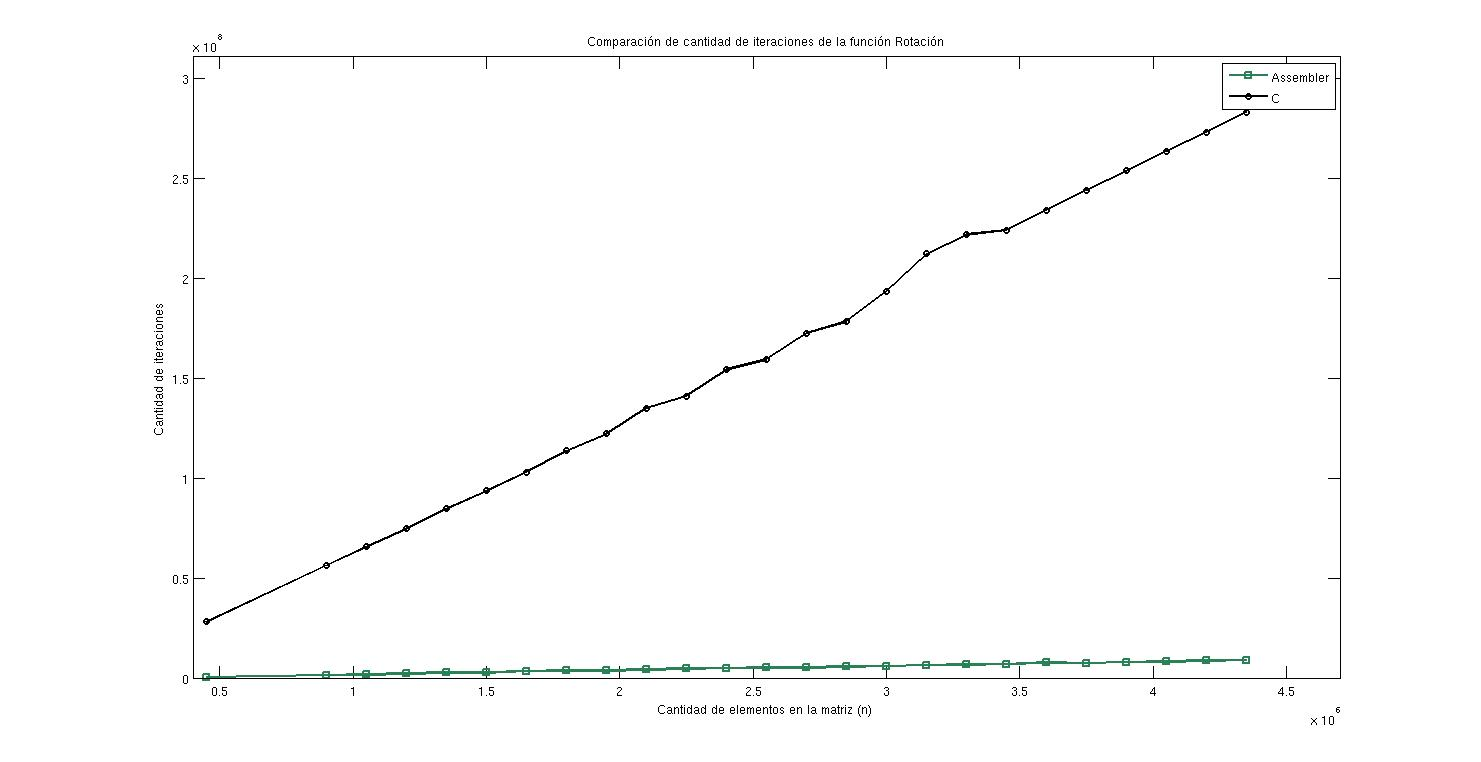
\includegraphics[width=500pt]{../imgs/comparacion_rotacion.jpg}
\end{center}
\end{figure}
\begin{figure}[H] %[h] Aqui [b] para button [t] para top
\begin{center}
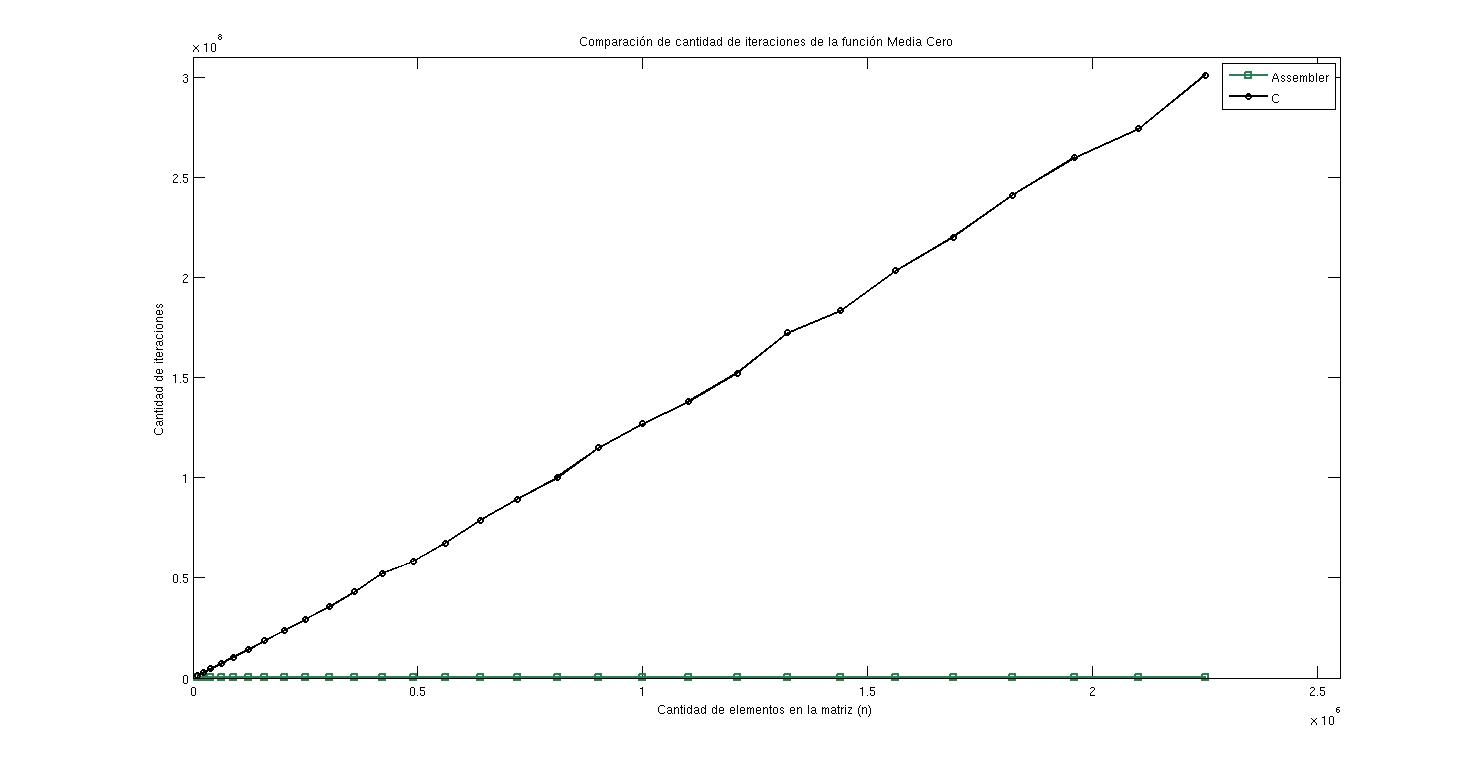
\includegraphics[width=500pt]{../imgs/comparacion_mediaCero.jpg}
\end{center}
\end{figure}
\begin{figure}[H] %[h] Aqui [b] para button [t] para top
\begin{center}
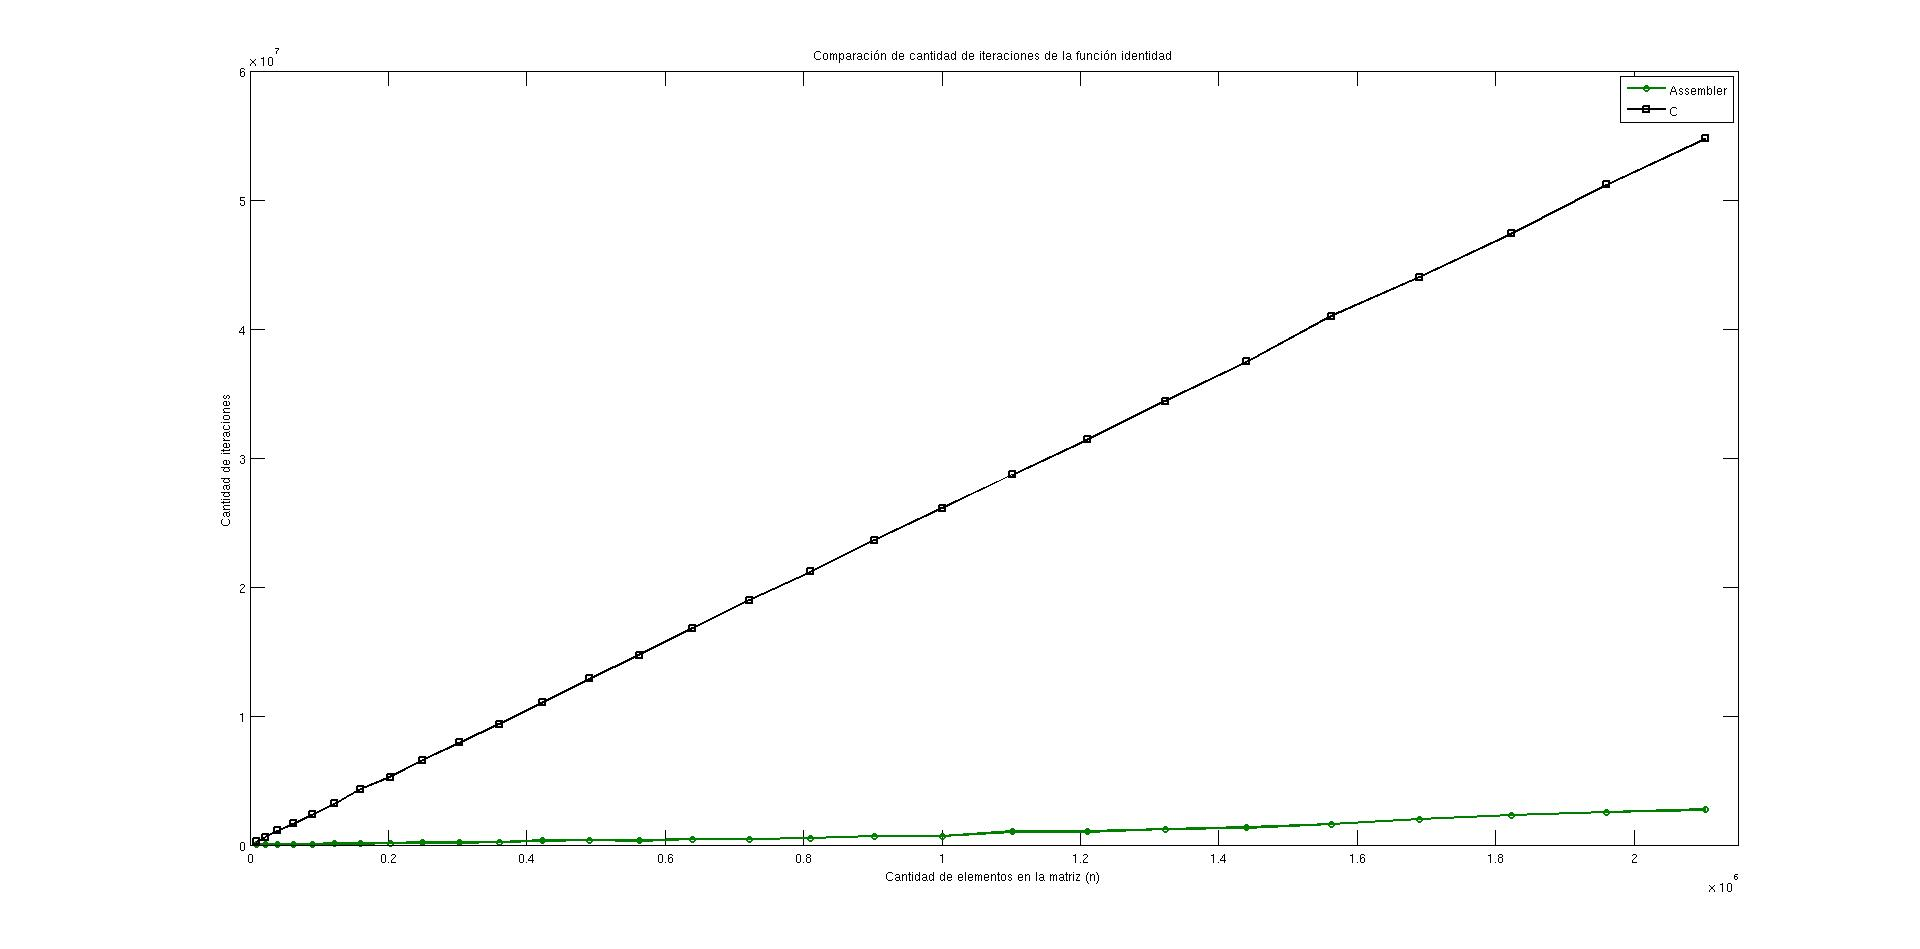
\includegraphics[width=500pt]{../imgs/comparacion_identidad.jpg}
\end{center}
\end{figure}

\begin{figure}[H] %[h] Aqui [b] para button [t] para top
\begin{center}
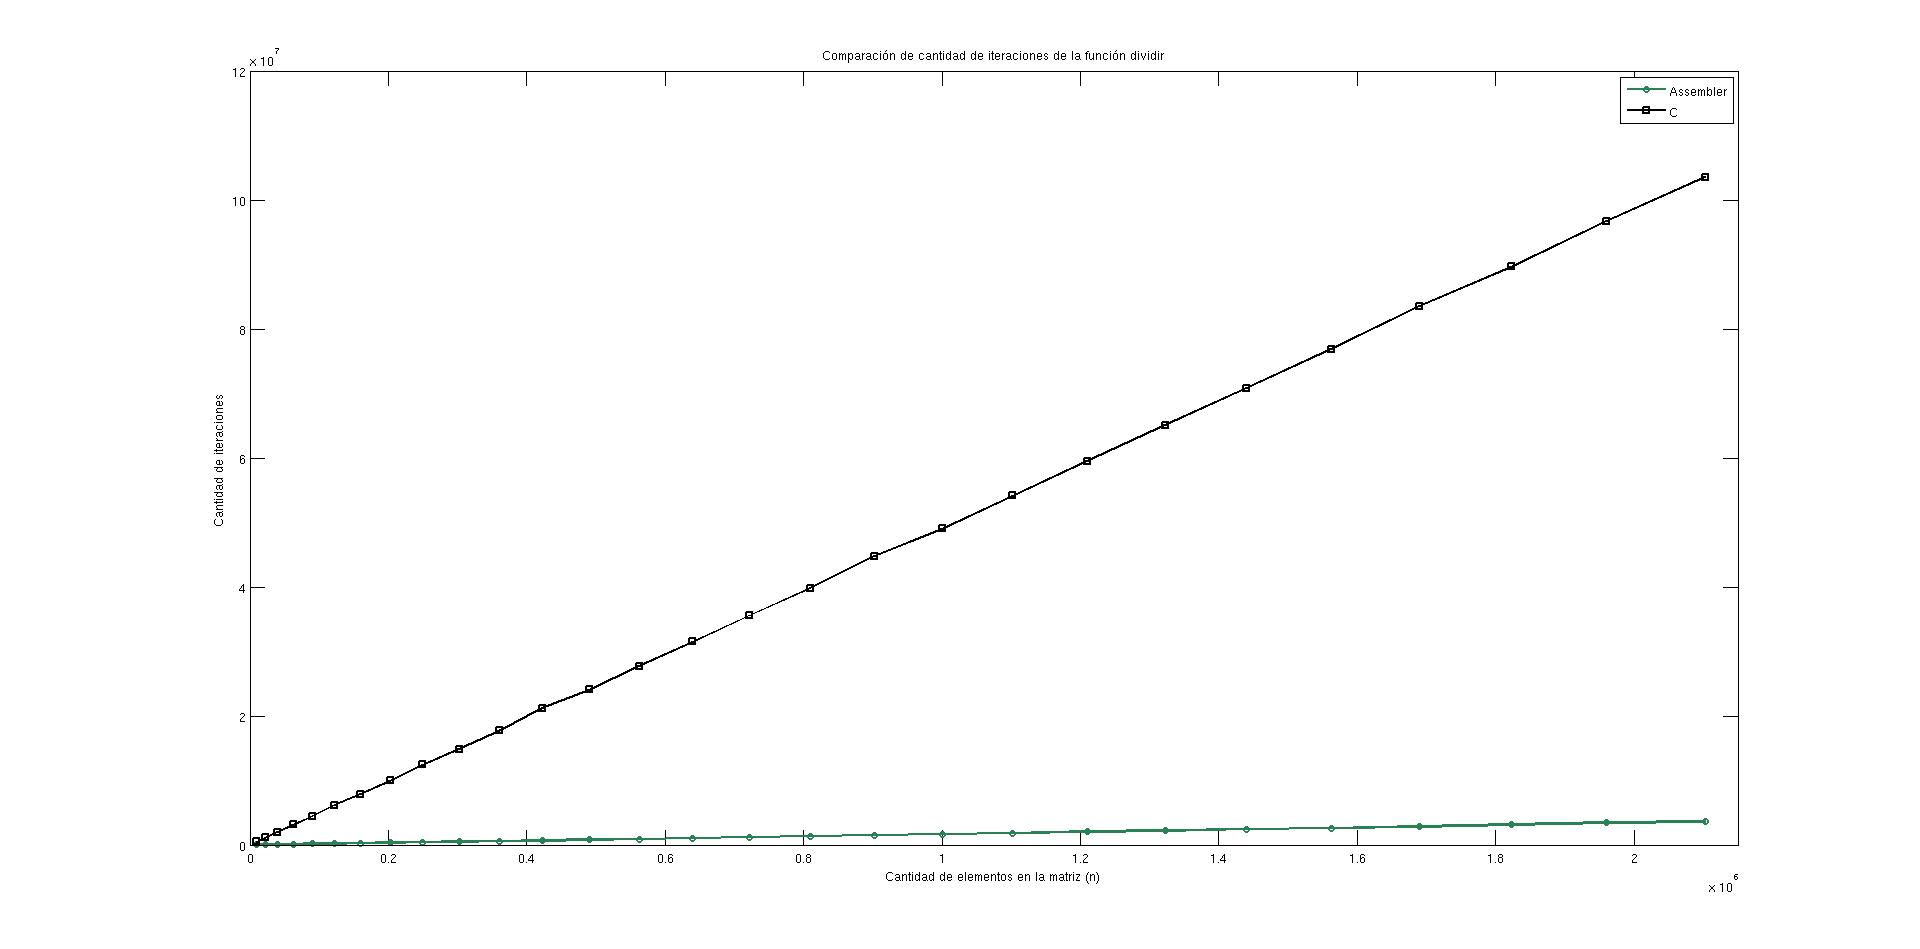
\includegraphics[width=500pt]{../imgs/comparacion_dividir.jpg}
\end{center}
\end{figure}

\begin{figure}[H] %[h] Aqui [b] para button [t] para top
\begin{center}
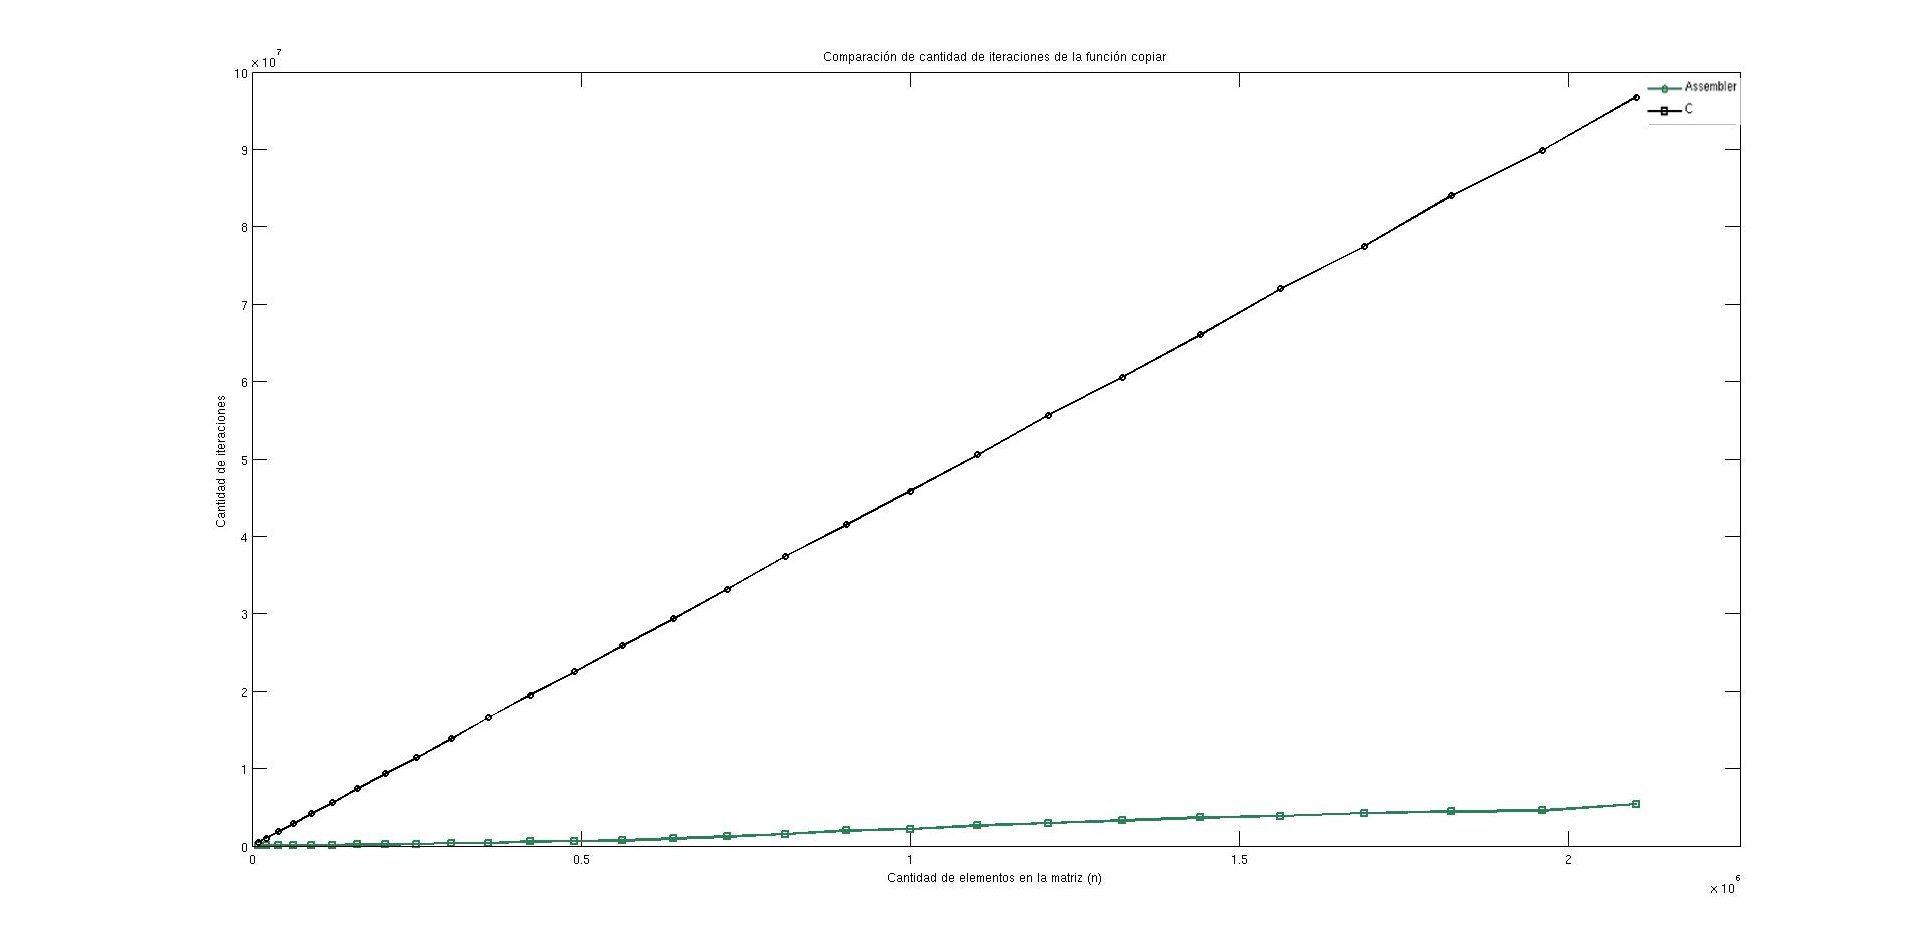
\includegraphics[width=500pt]{../imgs/comparacion_copiar.jpg}
\end{center}
\end{figure}

\begin{figure}[H] %[h] Aqui [b] para button [t] para top
\begin{center}
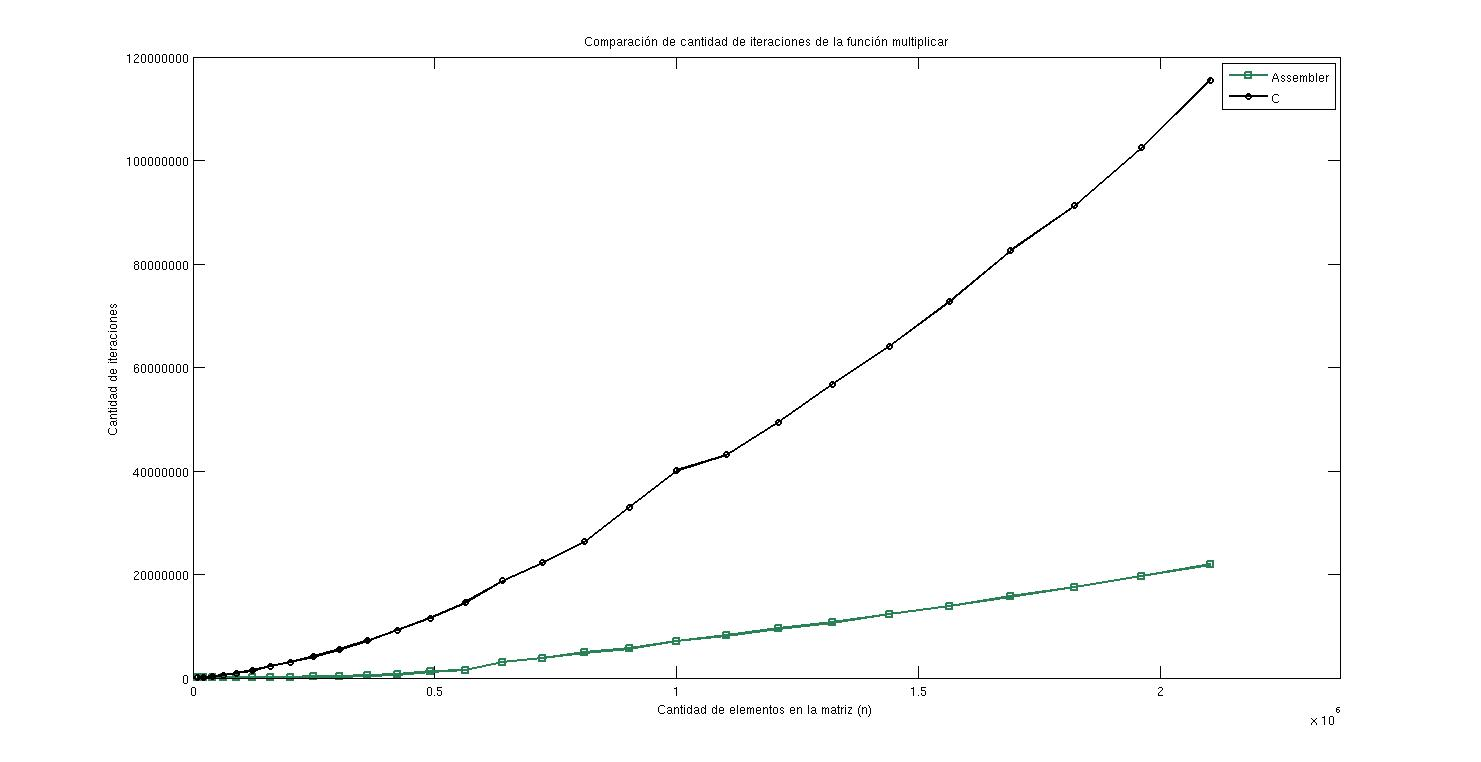
\includegraphics[width=500pt]{../imgs/comparacion_multiplicar.jpg}
\end{center}
\end{figure}

Dado que las funciones anteriores poseen una relación similar entre la cantidad de iteraciones de la función en $C$ y $Assembler$, decidimos analizarlas juntas con el fin de evitar redundancias en las explicaciones.
Al desensamblar las funciones en $C$, nos encontramos, en primer lugar, con las mismas características que se mencionaron anteriormente, siendo éstas las mayores responsables de la diferencia en la cantidad de ciclos y, por lo tanto, de la lentitud de la ejecución en $C$ respecto del $Assembler$. Éstas son los accesos a memoria tanto para almacenar como para consultar datos, las llamadas que producen los múltiples accesos a memoria para almacenar los valores de los registros y el procesamiento de un elemento a la vez. 
Por otro lado, nos encontramos con que el código en $C$ utiliza registros XMM a diferencia de que no los aprovecha a todos sino que los aplica únicamente para calcular desplazamientos y operaciones simples con $movss$, $mulss$ y $subss$. 

Por otro lado, nos percatamos de que algunas operaciones son reemplazadas por un conjunto de otras, por ejemplo, la función $sqrt$ es reemplazada por una serie de operaciones simples que aproximan el valor de la raíz.

Por último, concluimos que calidad no se relaciona con cantidad debido a que nuestro código $Assembler$ resulta más extenso que el desensamblado del $C$ pues este último consiste en una constante repetición de operaciones simples. En cambio, nuestro $Assembler$ realiza menos ciclos siendo cada uno de éstos más extenso por contener funciones que optimizan la cantidad de operaciones a realizar.

En lo que sigue, se puede ver un gráfico comparativo del tiempo que toma procesar la matriz en $C$ y en $Assembler$ en una computadora con 6GB de memoria RAM y un procesador Intel® Core™ i3-3120M CPU @ 2.50GHz × 4.
\begin{figure}[H] %[h] Aqui [b] para button [t] para top
\begin{center}
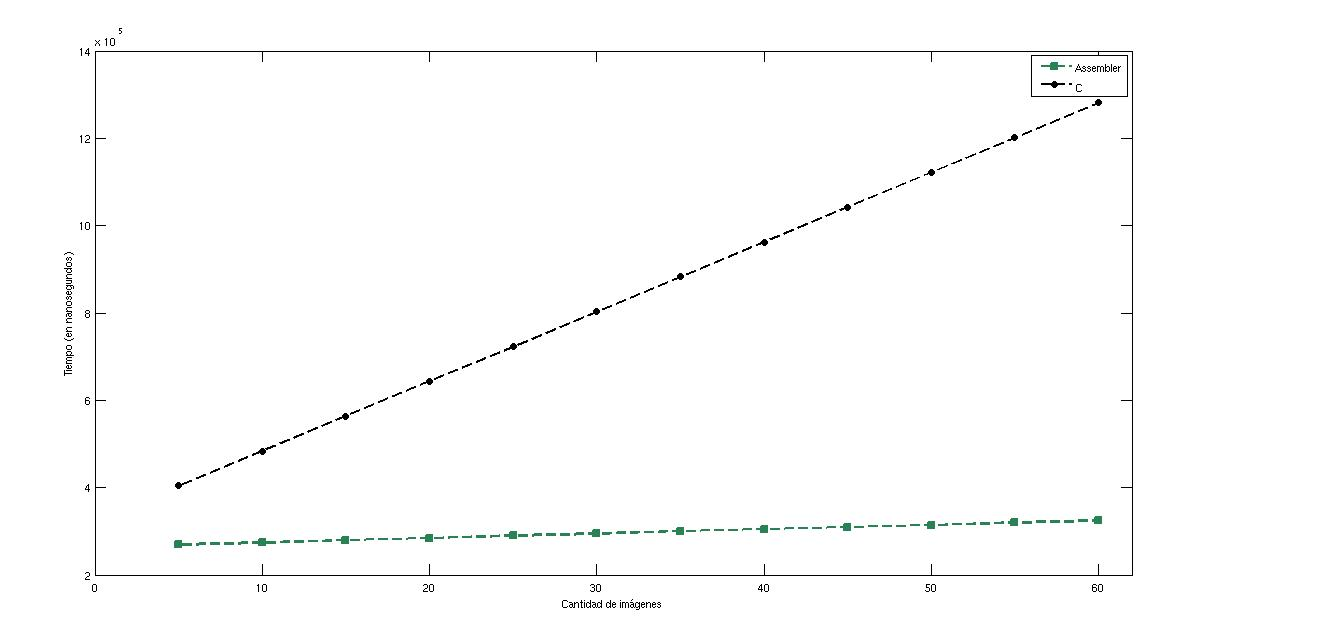
\includegraphics[width=540pt]{../imgs/comparacion_total.jpg}
\end{center}
\end{figure}

\section{Conclusi\'on}
Podemos concluir que las causas principales de que el código en $C$ sea más lento que el código $Assembler$ son que su ensamblado no utiliza instrucciones SIMD y que almacena todos los datos en la pila que son llamados en cada iteración. Esto significa que $C$ usa la FPU que es poco performante causando un aumento del tiempo de ejecución.\newline
A partir de aquí, podemos afirmar que realizar operaciones de a muchos bits a la vez, empaquetando y desempaquetando los datos, acelera enormemente el tiempo de ejecución de una función. Del mismo modo, los llamados a memoria dentro de los ciclos ralentizan la velocidad de ejecución enormemente.

\section{Referencias}
\begin{itemize}
\item BURDEN, RICHARD L. ; An\'alisis num\'erico, 7ma ed. 2002. M\'exico, Thomson Learning.
\item WATKINS, DAVID S. ; Understanding the QR Algorithm, 1982, SIAM Review
\item HENRY, GREG ; A parallel implementation of the nonsymmetric QR algorithm for distributed memory architectures, 2002, SIAM J. SCI. COMPUT.
\end{itemize}

\newpage
\end{document}
